%  MDPI Sensors submission.  Build: `make paper` from the repository root.
%  Every number in this manuscript is a \R{key} lookup into
%  generated/numbers.tex, which paper/scripts/make_numbers.py writes from the
%  experiment artifacts.  Do not type a result into this file by hand.
\documentclass[sensors,article,submit,moreauthors]{Definitions/mdpi}

\usepackage{tikz}
\usetikzlibrary{arrows.meta,positioning,calc}
% GENERATED by paper/scripts/make_numbers.py -- do not edit.
\makeatletter
\DeclareRobustCommand{\R}[1]{\ifcsname rnum@#1\endcsname\csname rnum@#1\endcsname\else\textbf{\textcolor{red}{??#1??}}\PackageWarning{numbers}{undefined number #1}\fi}
\expandafter\def\csname rnum@abl.cnn.AUC\endcsname{0.869}
\expandafter\def\csname rnum@abl.cnn.AUCCI\endcsname{[0.784, 0.933]}
\expandafter\def\csname rnum@abl.cnn.F1\endcsname{0.573}
\expandafter\def\csname rnum@abl.cnn.evRec\endcsname{0.821}
\expandafter\def\csname rnum@abl.cnn.evSpec\endcsname{0.764}
\expandafter\def\csname rnum@abl.cnnparams\endcsname{24{,}417}
\expandafter\def\csname rnum@abl.hgb.AUC\endcsname{0.893}
\expandafter\def\csname rnum@abl.hgb.AUCCI\endcsname{[0.829, 0.937]}
\expandafter\def\csname rnum@abl.hgb.F1\endcsname{0.663}
\expandafter\def\csname rnum@abl.hgb.evRec\endcsname{0.821}
\expandafter\def\csname rnum@abl.hgb.evSpec\endcsname{0.918}
\expandafter\def\csname rnum@abl.rfe.AUC\endcsname{0.900}
\expandafter\def\csname rnum@abl.rfe.AUCCI\endcsname{[0.829, 0.946]}
\expandafter\def\csname rnum@abl.rfe.F1\endcsname{0.649}
\expandafter\def\csname rnum@abl.rfe.evRec\endcsname{0.896}
\expandafter\def\csname rnum@abl.rfe.evSpec\endcsname{0.880}
\expandafter\def\csname rnum@abl.rocket.AUC\endcsname{0.890}
\expandafter\def\csname rnum@abl.rocket.AUCCI\endcsname{[0.826, 0.934]}
\expandafter\def\csname rnum@abl.rocket.F1\endcsname{0.612}
\expandafter\def\csname rnum@abl.rocket.evRec\endcsname{0.873}
\expandafter\def\csname rnum@abl.rocket.evSpec\endcsname{0.856}
\expandafter\def\csname rnum@asm.asleep.med\endcsname{40}
\expandafter\def\csname rnum@asm.asleep.p\endcsname{0.60}
\expandafter\def\csname rnum@asm.asleep.sig\endcsname{0.8}
\expandafter\def\csname rnum@asm.awake.med\endcsname{15}
\expandafter\def\csname rnum@asm.awake.p\endcsname{0.95}
\expandafter\def\csname rnum@asm.awake.sig\endcsname{0.8}
\expandafter\def\csname rnum@asm.care.med\endcsname{45}
\expandafter\def\csname rnum@asm.care.p\endcsname{0.80}
\expandafter\def\csname rnum@asm.care.sig\endcsname{0.8}
\expandafter\def\csname rnum@asm.emerg.med\endcsname{30}
\expandafter\def\csname rnum@asm.emerg.p\endcsname{0.99}
\expandafter\def\csname rnum@asm.emerg.sig\endcsname{0.5}
\expandafter\def\csname rnum@asm.loss\endcsname{0.02}
\expandafter\def\csname rnum@bench.direct.us\endcsname{260}
\expandafter\def\csname rnum@bench.duty\endcsname{0.010}
\expandafter\def\csname rnum@bench.forest.us\endcsname{0.27}
\expandafter\def\csname rnum@bench.macs\endcsname{140{,}448}
\expandafter\def\csname rnum@bench.scratch\endcsname{6{,}724}
\expandafter\def\csname rnum@bench.speedup\endcsname{2.0}
\expandafter\def\csname rnum@bench.trig\endcsname{140{,}448}
\expandafter\def\csname rnum@bench.us\endcsname{130}
\expandafter\def\csname rnum@bench.visits\endcsname{172}
\expandafter\def\csname rnum@burden.attenuation\endcsname{3.9}
\expandafter\def\csname rnum@burden.measured.careday\endcsname{175}
\expandafter\def\csname rnum@burden.measured.emergday\endcsname{52.8}
\expandafter\def\csname rnum@burden.measured.faday\endcsname{687}
\expandafter\def\csname rnum@burden.measured.fah\endcsname{28.6}
\expandafter\def\csname rnum@burden.preach\endcsname{25.4}
\expandafter\def\csname rnum@cfg.eventsamples\endcsname{401}
\expandafter\def\csname rnum@cfg.eventseconds\endcsname{7.83}
\expandafter\def\csname rnum@cfg.maxfar\endcsname{5}
\expandafter\def\csname rnum@cfg.nfeat\endcsname{159}
\expandafter\def\csname rnum@cfg.nsel\endcsname{20}
\expandafter\def\csname rnum@cfg.refractory\endcsname{60}
\expandafter\def\csname rnum@cfg.stride\endcsname{1.3}
\expandafter\def\csname rnum@cfg.stridesamples\endcsname{67}
\expandafter\def\csname rnum@cfg.window\endcsname{2.6}
\expandafter\def\csname rnum@cfg.winsamples\endcsname{133}
\expandafter\def\csname rnum@cmp.base.dAUC\endcsname{$-$0.008}
\expandafter\def\csname rnum@cmp.base.dAUCCI\endcsname{[$-$0.034, 0.015]}
\expandafter\def\csname rnum@cmp.base.dF1\endcsname{$-$0.067}
\expandafter\def\csname rnum@cmp.base.dF1CI\endcsname{[$-$0.106, $-$0.023]}
\expandafter\def\csname rnum@cmp.base.mcB\endcsname{12}
\expandafter\def\csname rnum@cmp.base.mcC\endcsname{1}
\expandafter\def\csname rnum@cmp.base.mcP\endcsname{0.003}
\expandafter\def\csname rnum@cmp.base.pAUC\endcsname{0.498}
\expandafter\def\csname rnum@cmp.base.pF1\endcsname{0.010}
\expandafter\def\csname rnum@cmp.base.pWil\endcsname{0.052}
\expandafter\def\csname rnum@cmp.lr.dAUC\endcsname{0.013}
\expandafter\def\csname rnum@cmp.lr.dAUCCI\endcsname{[0.002, 0.030]}
\expandafter\def\csname rnum@cmp.lr.dF1\endcsname{0.007}
\expandafter\def\csname rnum@cmp.lr.dF1CI\endcsname{[$-$0.016, 0.032]}
\expandafter\def\csname rnum@cmp.lr.mcB\endcsname{13}
\expandafter\def\csname rnum@cmp.lr.mcC\endcsname{7}
\expandafter\def\csname rnum@cmp.lr.mcP\endcsname{0.263}
\expandafter\def\csname rnum@cmp.lr.pAUC\endcsname{0.130}
\expandafter\def\csname rnum@cmp.lr.pF1\endcsname{1.000}
\expandafter\def\csname rnum@cmp.lr.pWil\endcsname{0.572}
\expandafter\def\csname rnum@cmp.nb.dAUC\endcsname{$-$0.013}
\expandafter\def\csname rnum@cmp.nb.dAUCCI\endcsname{[$-$0.032, 0.003]}
\expandafter\def\csname rnum@cmp.nb.dF1\endcsname{$-$0.040}
\expandafter\def\csname rnum@cmp.nb.dF1CI\endcsname{[$-$0.070, $-$0.001]}
\expandafter\def\csname rnum@cmp.nb.mcB\endcsname{19}
\expandafter\def\csname rnum@cmp.nb.mcC\endcsname{1}
\expandafter\def\csname rnum@cmp.nb.mcP\endcsname{0.0000}
\expandafter\def\csname rnum@cmp.nb.pAUC\endcsname{0.420}
\expandafter\def\csname rnum@cmp.nb.pF1\endcsname{0.180}
\expandafter\def\csname rnum@cmp.nb.pWil\endcsname{0.829}
\expandafter\def\csname rnum@cmp.rf.dAUC\endcsname{$-$0.004}
\expandafter\def\csname rnum@cmp.rf.dAUCCI\endcsname{[$-$0.010, 0.002]}
\expandafter\def\csname rnum@cmp.rf.dF1\endcsname{0.006}
\expandafter\def\csname rnum@cmp.rf.dF1CI\endcsname{[$-$0.029, 0.040]}
\expandafter\def\csname rnum@cmp.rf.mcB\endcsname{3}
\expandafter\def\csname rnum@cmp.rf.mcC\endcsname{7}
\expandafter\def\csname rnum@cmp.rf.mcP\endcsname{0.344}
\expandafter\def\csname rnum@cmp.rf.pAUC\endcsname{0.498}
\expandafter\def\csname rnum@cmp.rf.pF1\endcsname{1.000}
\expandafter\def\csname rnum@cmp.rf.pWil\endcsname{0.811}
\expandafter\def\csname rnum@cmp.svm.dAUC\endcsname{$-$0.024}
\expandafter\def\csname rnum@cmp.svm.dAUCCI\endcsname{[$-$0.062, 0.006]}
\expandafter\def\csname rnum@cmp.svm.dF1\endcsname{0.012}
\expandafter\def\csname rnum@cmp.svm.dF1CI\endcsname{[$-$0.009, 0.041]}
\expandafter\def\csname rnum@cmp.svm.mcB\endcsname{6}
\expandafter\def\csname rnum@cmp.svm.mcC\endcsname{2}
\expandafter\def\csname rnum@cmp.svm.mcP\endcsname{0.289}
\expandafter\def\csname rnum@cmp.svm.pAUC\endcsname{0.498}
\expandafter\def\csname rnum@cmp.svm.pF1\endcsname{0.831}
\expandafter\def\csname rnum@cmp.svm.pWil\endcsname{0.259}
\expandafter\def\csname rnum@cont.base.r0.epdet\endcsname{58}
\expandafter\def\csname rnum@cont.base.r0.epn\endcsname{78}
\expandafter\def\csname rnum@cont.base.r0.epsens\endcsname{0.744}
\expandafter\def\csname rnum@cont.base.r0.epsensCI\endcsname{[0.623, 0.855]}
\expandafter\def\csname rnum@cont.base.r0.exposure\endcsname{0.63}
\expandafter\def\csname rnum@cont.base.r0.fa\endcsname{58}
\expandafter\def\csname rnum@cont.base.r0.fah\endcsname{92.2}
\expandafter\def\csname rnum@cont.base.r0.fahBootCI\endcsname{[33.3, 180.6]}
\expandafter\def\csname rnum@cont.base.r0.fahCI\endcsname{[70.0, 119.2]}
\expandafter\def\csname rnum@cont.base.r0.lat\endcsname{2.9}
\expandafter\def\csname rnum@cont.base.r0.spindet\endcsname{81}
\expandafter\def\csname rnum@cont.base.r0.spinn\endcsname{135}
\expandafter\def\csname rnum@cont.base.r0.spinsens\endcsname{0.600}
\expandafter\def\csname rnum@cont.base.r0.spinsensCI\endcsname{[0.477, 0.724]}
\expandafter\def\csname rnum@cont.base.r60.epdet\endcsname{50}
\expandafter\def\csname rnum@cont.base.r60.epn\endcsname{78}
\expandafter\def\csname rnum@cont.base.r60.epsens\endcsname{0.641}
\expandafter\def\csname rnum@cont.base.r60.epsensCI\endcsname{[0.506, 0.771]}
\expandafter\def\csname rnum@cont.base.r60.exposure\endcsname{0.63}
\expandafter\def\csname rnum@cont.base.r60.fa\endcsname{15}
\expandafter\def\csname rnum@cont.base.r60.fah\endcsname{23.8}
\expandafter\def\csname rnum@cont.base.r60.fahBootCI\endcsname{[10.1, 43.9]}
\expandafter\def\csname rnum@cont.base.r60.fahCI\endcsname{[13.3, 39.3]}
\expandafter\def\csname rnum@cont.base.r60.lat\endcsname{2.9}
\expandafter\def\csname rnum@cont.base.r60.spindet\endcsname{50}
\expandafter\def\csname rnum@cont.base.r60.spinn\endcsname{135}
\expandafter\def\csname rnum@cont.base.r60.spinsens\endcsname{0.370}
\expandafter\def\csname rnum@cont.base.r60.spinsensCI\endcsname{[0.277, 0.466]}
\expandafter\def\csname rnum@cont.base.s0.epdet\endcsname{61}
\expandafter\def\csname rnum@cont.base.s0.epn\endcsname{78}
\expandafter\def\csname rnum@cont.base.s0.epsens\endcsname{0.782}
\expandafter\def\csname rnum@cont.base.s0.epsensCI\endcsname{[0.667, 0.885]}
\expandafter\def\csname rnum@cont.base.s0.exposure\endcsname{0.63}
\expandafter\def\csname rnum@cont.base.s0.fa\endcsname{50}
\expandafter\def\csname rnum@cont.base.s0.fah\endcsname{79.5}
\expandafter\def\csname rnum@cont.base.s0.fahBootCI\endcsname{[35.6, 143.2]}
\expandafter\def\csname rnum@cont.base.s0.fahCI\endcsname{[59.0, 104.8]}
\expandafter\def\csname rnum@cont.base.s0.lat\endcsname{2.8}
\expandafter\def\csname rnum@cont.base.s0.spindet\endcsname{89}
\expandafter\def\csname rnum@cont.base.s0.spinn\endcsname{135}
\expandafter\def\csname rnum@cont.base.s0.spinsens\endcsname{0.659}
\expandafter\def\csname rnum@cont.base.s0.spinsensCI\endcsname{[0.529, 0.785]}
\expandafter\def\csname rnum@cont.base.s60.epdet\endcsname{54}
\expandafter\def\csname rnum@cont.base.s60.epn\endcsname{78}
\expandafter\def\csname rnum@cont.base.s60.epsens\endcsname{0.692}
\expandafter\def\csname rnum@cont.base.s60.epsensCI\endcsname{[0.574, 0.803]}
\expandafter\def\csname rnum@cont.base.s60.exposure\endcsname{0.63}
\expandafter\def\csname rnum@cont.base.s60.fa\endcsname{15}
\expandafter\def\csname rnum@cont.base.s60.fah\endcsname{23.8}
\expandafter\def\csname rnum@cont.base.s60.fahBootCI\endcsname{[11.8, 39.8]}
\expandafter\def\csname rnum@cont.base.s60.fahCI\endcsname{[13.3, 39.3]}
\expandafter\def\csname rnum@cont.base.s60.lat\endcsname{2.8}
\expandafter\def\csname rnum@cont.base.s60.spindet\endcsname{54}
\expandafter\def\csname rnum@cont.base.s60.spinn\endcsname{135}
\expandafter\def\csname rnum@cont.base.s60.spinsens\endcsname{0.400}
\expandafter\def\csname rnum@cont.base.s60.spinsensCI\endcsname{[0.312, 0.489]}
\expandafter\def\csname rnum@cont.base.tol0.fah\endcsname{92.2}
\expandafter\def\csname rnum@cont.base.tol0.spinsens\endcsname{0.600}
\expandafter\def\csname rnum@cont.base.tol10.fah\endcsname{90.3}
\expandafter\def\csname rnum@cont.base.tol10.spinsens\endcsname{0.674}
\expandafter\def\csname rnum@cont.base.tol20.fah\endcsname{81.4}
\expandafter\def\csname rnum@cont.base.tol20.spinsens\endcsname{0.711}
\expandafter\def\csname rnum@cont.base.tol2p5.fah\endcsname{85.9}
\expandafter\def\csname rnum@cont.base.tol2p5.spinsens\endcsname{0.644}
\expandafter\def\csname rnum@cont.base.tol5.fah\endcsname{88.3}
\expandafter\def\csname rnum@cont.base.tol5.spinsens\endcsname{0.644}
\expandafter\def\csname rnum@cont.ratio.curated\endcsname{2.7}
\expandafter\def\csname rnum@cont.rf.r0.epdet\endcsname{59}
\expandafter\def\csname rnum@cont.rf.r0.epn\endcsname{78}
\expandafter\def\csname rnum@cont.rf.r0.epsens\endcsname{0.756}
\expandafter\def\csname rnum@cont.rf.r0.epsensCI\endcsname{[0.645, 0.860]}
\expandafter\def\csname rnum@cont.rf.r0.exposure\endcsname{0.63}
\expandafter\def\csname rnum@cont.rf.r0.fa\endcsname{37}
\expandafter\def\csname rnum@cont.rf.r0.fah\endcsname{58.8}
\expandafter\def\csname rnum@cont.rf.r0.fahBootCI\endcsname{[26.5, 108.7]}
\expandafter\def\csname rnum@cont.rf.r0.fahCI\endcsname{[41.4, 81.1]}
\expandafter\def\csname rnum@cont.rf.r0.lat\endcsname{2.9}
\expandafter\def\csname rnum@cont.rf.r0.spindet\endcsname{98}
\expandafter\def\csname rnum@cont.rf.r0.spinn\endcsname{135}
\expandafter\def\csname rnum@cont.rf.r0.spinsens\endcsname{0.726}
\expandafter\def\csname rnum@cont.rf.r0.spinsensCI\endcsname{[0.578, 0.847]}
\expandafter\def\csname rnum@cont.rf.r60.epdet\endcsname{53}
\expandafter\def\csname rnum@cont.rf.r60.epn\endcsname{78}
\expandafter\def\csname rnum@cont.rf.r60.epsens\endcsname{0.679}
\expandafter\def\csname rnum@cont.rf.r60.epsensCI\endcsname{[0.570, 0.795]}
\expandafter\def\csname rnum@cont.rf.r60.exposure\endcsname{0.63}
\expandafter\def\csname rnum@cont.rf.r60.fa\endcsname{16}
\expandafter\def\csname rnum@cont.rf.r60.fah\endcsname{25.4}
\expandafter\def\csname rnum@cont.rf.r60.fahBootCI\endcsname{[12.1, 43.5]}
\expandafter\def\csname rnum@cont.rf.r60.fahCI\endcsname{[14.5, 41.3]}
\expandafter\def\csname rnum@cont.rf.r60.lat\endcsname{3.1}
\expandafter\def\csname rnum@cont.rf.r60.spindet\endcsname{53}
\expandafter\def\csname rnum@cont.rf.r60.spinn\endcsname{135}
\expandafter\def\csname rnum@cont.rf.r60.spinsens\endcsname{0.393}
\expandafter\def\csname rnum@cont.rf.r60.spinsensCI\endcsname{[0.308, 0.482]}
\expandafter\def\csname rnum@cont.rf.s0.epdet\endcsname{58}
\expandafter\def\csname rnum@cont.rf.s0.epn\endcsname{78}
\expandafter\def\csname rnum@cont.rf.s0.epsens\endcsname{0.744}
\expandafter\def\csname rnum@cont.rf.s0.epsensCI\endcsname{[0.635, 0.846]}
\expandafter\def\csname rnum@cont.rf.s0.exposure\endcsname{0.63}
\expandafter\def\csname rnum@cont.rf.s0.fa\endcsname{29}
\expandafter\def\csname rnum@cont.rf.s0.fah\endcsname{46.1}
\expandafter\def\csname rnum@cont.rf.s0.fahBootCI\endcsname{[22.4, 81.2]}
\expandafter\def\csname rnum@cont.rf.s0.fahCI\endcsname{[30.9, 66.2]}
\expandafter\def\csname rnum@cont.rf.s0.lat\endcsname{2.9}
\expandafter\def\csname rnum@cont.rf.s0.spindet\endcsname{95}
\expandafter\def\csname rnum@cont.rf.s0.spinn\endcsname{135}
\expandafter\def\csname rnum@cont.rf.s0.spinsens\endcsname{0.704}
\expandafter\def\csname rnum@cont.rf.s0.spinsensCI\endcsname{[0.557, 0.824]}
\expandafter\def\csname rnum@cont.rf.s60.epdet\endcsname{53}
\expandafter\def\csname rnum@cont.rf.s60.epn\endcsname{78}
\expandafter\def\csname rnum@cont.rf.s60.epsens\endcsname{0.679}
\expandafter\def\csname rnum@cont.rf.s60.epsensCI\endcsname{[0.575, 0.789]}
\expandafter\def\csname rnum@cont.rf.s60.exposure\endcsname{0.63}
\expandafter\def\csname rnum@cont.rf.s60.fa\endcsname{13}
\expandafter\def\csname rnum@cont.rf.s60.fah\endcsname{20.7}
\expandafter\def\csname rnum@cont.rf.s60.fahBootCI\endcsname{[9.6, 35.8]}
\expandafter\def\csname rnum@cont.rf.s60.fahCI\endcsname{[11.0, 35.3]}
\expandafter\def\csname rnum@cont.rf.s60.lat\endcsname{2.9}
\expandafter\def\csname rnum@cont.rf.s60.spindet\endcsname{53}
\expandafter\def\csname rnum@cont.rf.s60.spinn\endcsname{135}
\expandafter\def\csname rnum@cont.rf.s60.spinsens\endcsname{0.393}
\expandafter\def\csname rnum@cont.rf.s60.spinsensCI\endcsname{[0.309, 0.481]}
\expandafter\def\csname rnum@cont.rf.tol0.fah\endcsname{58.8}
\expandafter\def\csname rnum@cont.rf.tol0.spinsens\endcsname{0.726}
\expandafter\def\csname rnum@cont.rf.tol10.fah\endcsname{46.2}
\expandafter\def\csname rnum@cont.rf.tol10.spinsens\endcsname{0.763}
\expandafter\def\csname rnum@cont.rf.tol20.fah\endcsname{43.2}
\expandafter\def\csname rnum@cont.rf.tol20.spinsens\endcsname{0.785}
\expandafter\def\csname rnum@cont.rf.tol2p5.fah\endcsname{51.9}
\expandafter\def\csname rnum@cont.rf.tol2p5.spinsens\endcsname{0.756}
\expandafter\def\csname rnum@cont.rf.tol5.fah\endcsname{49.0}
\expandafter\def\csname rnum@cont.rf.tol5.spinsens\endcsname{0.756}
\expandafter\def\csname rnum@cont.rfe.r0.epdet\endcsname{56}
\expandafter\def\csname rnum@cont.rfe.r0.epn\endcsname{78}
\expandafter\def\csname rnum@cont.rfe.r0.epsens\endcsname{0.718}
\expandafter\def\csname rnum@cont.rfe.r0.epsensCI\endcsname{[0.588, 0.838]}
\expandafter\def\csname rnum@cont.rfe.r0.exposure\endcsname{0.63}
\expandafter\def\csname rnum@cont.rfe.r0.fa\endcsname{38}
\expandafter\def\csname rnum@cont.rfe.r0.fah\endcsname{60.4}
\expandafter\def\csname rnum@cont.rfe.r0.fahBootCI\endcsname{[32.7, 103.1]}
\expandafter\def\csname rnum@cont.rfe.r0.fahCI\endcsname{[42.7, 82.9]}
\expandafter\def\csname rnum@cont.rfe.r0.lat\endcsname{3.9}
\expandafter\def\csname rnum@cont.rfe.r0.spindet\endcsname{84}
\expandafter\def\csname rnum@cont.rfe.r0.spinn\endcsname{135}
\expandafter\def\csname rnum@cont.rfe.r0.spinsens\endcsname{0.622}
\expandafter\def\csname rnum@cont.rfe.r0.spinsensCI\endcsname{[0.500, 0.738]}
\expandafter\def\csname rnum@cont.rfe.r60.epdet\endcsname{50}
\expandafter\def\csname rnum@cont.rfe.r60.epn\endcsname{78}
\expandafter\def\csname rnum@cont.rfe.r60.epsens\endcsname{0.641}
\expandafter\def\csname rnum@cont.rfe.r60.epsensCI\endcsname{[0.518, 0.758]}
\expandafter\def\csname rnum@cont.rfe.r60.exposure\endcsname{0.63}
\expandafter\def\csname rnum@cont.rfe.r60.fa\endcsname{18}
\expandafter\def\csname rnum@cont.rfe.r60.fah\endcsname{28.6}
\expandafter\def\csname rnum@cont.rfe.r60.fahBootCI\endcsname{[16.2, 48.6]}
\expandafter\def\csname rnum@cont.rfe.r60.fahCI\endcsname{[17.0, 45.2]}
\expandafter\def\csname rnum@cont.rfe.r60.lat\endcsname{3.9}
\expandafter\def\csname rnum@cont.rfe.r60.spindet\endcsname{50}
\expandafter\def\csname rnum@cont.rfe.r60.spinn\endcsname{135}
\expandafter\def\csname rnum@cont.rfe.r60.spinsens\endcsname{0.370}
\expandafter\def\csname rnum@cont.rfe.r60.spinsensCI\endcsname{[0.289, 0.467]}
\expandafter\def\csname rnum@cont.rfe.s0.epdet\endcsname{56}
\expandafter\def\csname rnum@cont.rfe.s0.epn\endcsname{78}
\expandafter\def\csname rnum@cont.rfe.s0.epsens\endcsname{0.718}
\expandafter\def\csname rnum@cont.rfe.s0.epsensCI\endcsname{[0.579, 0.846]}
\expandafter\def\csname rnum@cont.rfe.s0.exposure\endcsname{0.63}
\expandafter\def\csname rnum@cont.rfe.s0.fa\endcsname{33}
\expandafter\def\csname rnum@cont.rfe.s0.fah\endcsname{52.5}
\expandafter\def\csname rnum@cont.rfe.s0.fahBootCI\endcsname{[25.9, 91.4]}
\expandafter\def\csname rnum@cont.rfe.s0.fahCI\endcsname{[36.1, 73.7]}
\expandafter\def\csname rnum@cont.rfe.s0.lat\endcsname{4.1}
\expandafter\def\csname rnum@cont.rfe.s0.spindet\endcsname{79}
\expandafter\def\csname rnum@cont.rfe.s0.spinn\endcsname{135}
\expandafter\def\csname rnum@cont.rfe.s0.spinsens\endcsname{0.585}
\expandafter\def\csname rnum@cont.rfe.s0.spinsensCI\endcsname{[0.462, 0.693]}
\expandafter\def\csname rnum@cont.rfe.s60.epdet\endcsname{52}
\expandafter\def\csname rnum@cont.rfe.s60.epn\endcsname{78}
\expandafter\def\csname rnum@cont.rfe.s60.epsens\endcsname{0.667}
\expandafter\def\csname rnum@cont.rfe.s60.epsensCI\endcsname{[0.534, 0.789]}
\expandafter\def\csname rnum@cont.rfe.s60.exposure\endcsname{0.63}
\expandafter\def\csname rnum@cont.rfe.s60.fa\endcsname{14}
\expandafter\def\csname rnum@cont.rfe.s60.fah\endcsname{22.3}
\expandafter\def\csname rnum@cont.rfe.s60.fahBootCI\endcsname{[12.0, 38.6]}
\expandafter\def\csname rnum@cont.rfe.s60.fahCI\endcsname{[12.2, 37.3]}
\expandafter\def\csname rnum@cont.rfe.s60.lat\endcsname{4.2}
\expandafter\def\csname rnum@cont.rfe.s60.spindet\endcsname{53}
\expandafter\def\csname rnum@cont.rfe.s60.spinn\endcsname{135}
\expandafter\def\csname rnum@cont.rfe.s60.spinsens\endcsname{0.393}
\expandafter\def\csname rnum@cont.rfe.s60.spinsensCI\endcsname{[0.308, 0.479]}
\expandafter\def\csname rnum@cont.rfe.tol0.fah\endcsname{60.4}
\expandafter\def\csname rnum@cont.rfe.tol0.spinsens\endcsname{0.622}
\expandafter\def\csname rnum@cont.rfe.tol10.fah\endcsname{46.2}
\expandafter\def\csname rnum@cont.rfe.tol10.spinsens\endcsname{0.741}
\expandafter\def\csname rnum@cont.rfe.tol20.fah\endcsname{40.7}
\expandafter\def\csname rnum@cont.rfe.tol20.spinsens\endcsname{0.756}
\expandafter\def\csname rnum@cont.rfe.tol2p5.fah\endcsname{44.8}
\expandafter\def\csname rnum@cont.rfe.tol2p5.spinsens\endcsname{0.719}
\expandafter\def\csname rnum@cont.rfe.tol5.fah\endcsname{45.1}
\expandafter\def\csname rnum@cont.rfe.tol5.spinsens\endcsname{0.719}
\expandafter\def\csname rnum@ds.durmax\endcsname{5.29}
\expandafter\def\csname rnum@ds.durmedian\endcsname{2.46}
\expandafter\def\csname rnum@ds.durmin\endcsname{1.00}
\expandafter\def\csname rnum@ds.eventgroups\endcsname{32}
\expandafter\def\csname rnum@ds.events\endcsname{342}
\expandafter\def\csname rnum@ds.files\endcsname{78}
\expandafter\def\csname rnum@ds.fs\endcsname{51.2}
\expandafter\def\csname rnum@ds.groups\endcsname{33}
\expandafter\def\csname rnum@ds.hours\endcsname{0.82}
\expandafter\def\csname rnum@ds.minutes\endcsname{49}
\expandafter\def\csname rnum@ds.negevents\endcsname{208}
\expandafter\def\csname rnum@ds.posevents\endcsname{134}
\expandafter\def\csname rnum@ds.poswindows\endcsname{257}
\expandafter\def\csname rnum@ds.seconds\endcsname{2{,}937}
\expandafter\def\csname rnum@ds.sessions\endcsname{3}
\expandafter\def\csname rnum@ds.spins\endcsname{135}
\expandafter\def\csname rnum@ds.spinseconds\endcsname{340.6}
\expandafter\def\csname rnum@ds.streams\endcsname{78}
\expandafter\def\csname rnum@ds.windows\endcsname{1{,}710}
\expandafter\def\csname rnum@esc.hb\endcsname{15}
\expandafter\def\csname rnum@esc.t1\endcsname{60}
\expandafter\def\csname rnum@esc.t2\endcsname{120}
\expandafter\def\csname rnum@esc.w\endcsname{60}
\expandafter\def\csname rnum@fam.accelonly.AUC\endcsname{0.852}
\expandafter\def\csname rnum@fam.accelonly.F1\endcsname{0.535}
\expandafter\def\csname rnum@fam.accelonly.evRec\endcsname{0.881}
\expandafter\def\csname rnum@fam.accelonly.n\endcsname{75}
\expandafter\def\csname rnum@fam.all159.AUC\endcsname{0.900}
\expandafter\def\csname rnum@fam.all159.F1\endcsname{0.649}
\expandafter\def\csname rnum@fam.all159.evRec\endcsname{0.896}
\expandafter\def\csname rnum@fam.all159.n\endcsname{159}
\expandafter\def\csname rnum@fam.gyromagnitudeonly.AUC\endcsname{0.906}
\expandafter\def\csname rnum@fam.gyromagnitudeonly.F1\endcsname{0.709}
\expandafter\def\csname rnum@fam.gyromagnitudeonly.evRec\endcsname{0.873}
\expandafter\def\csname rnum@fam.gyromagnitudeonly.n\endcsname{18}
\expandafter\def\csname rnum@fam.gyroonly.AUC\endcsname{0.892}
\expandafter\def\csname rnum@fam.gyroonly.F1\endcsname{0.668}
\expandafter\def\csname rnum@fam.gyroonly.evRec\endcsname{0.896}
\expandafter\def\csname rnum@fam.gyroonly.n\endcsname{75}
\expandafter\def\csname rnum@fam.magnitudesonly.AUC\endcsname{0.901}
\expandafter\def\csname rnum@fam.magnitudesonly.F1\endcsname{0.690}
\expandafter\def\csname rnum@fam.magnitudesonly.evRec\endcsname{0.866}
\expandafter\def\csname rnum@fam.magnitudesonly.n\endcsname{36}
\expandafter\def\csname rnum@fam.peraxisonly.AUC\endcsname{0.892}
\expandafter\def\csname rnum@fam.peraxisonly.F1\endcsname{0.645}
\expandafter\def\csname rnum@fam.peraxisonly.evRec\endcsname{0.896}
\expandafter\def\csname rnum@fam.peraxisonly.n\endcsname{123}
\expandafter\def\csname rnum@front.aucmax\endcsname{0.901}
\expandafter\def\csname rnum@front.aucmin\endcsname{0.876}
\expandafter\def\csname rnum@front.n\endcsname{30}
\expandafter\def\csname rnum@front.shipped.auc\endcsname{0.900}
\expandafter\def\csname rnum@front.shipped.kib\endcsname{39.4}
\expandafter\def\csname rnum@front.small.auc\endcsname{0.894}
\expandafter\def\csname rnum@front.small.depth\endcsname{6}
\expandafter\def\csname rnum@front.small.kib\endcsname{7.0}
\expandafter\def\csname rnum@front.small.trees\endcsname{8}
\expandafter\def\csname rnum@fw.checks\endcsname{240}
\expandafter\def\csname rnum@fw.failures\endcsname{0}
\expandafter\def\csname rnum@fw.featerr\endcsname{$3.0\times10^{-3}$}
\expandafter\def\csname rnum@fw.k\endcsname{2}
\expandafter\def\csname rnum@fw.kib\endcsname{39.4}
\expandafter\def\csname rnum@fw.n\endcsname{4}
\expandafter\def\csname rnum@fw.nodes\endcsname{2{,}880}
\expandafter\def\csname rnum@fw.probaerr\endcsname{$1.8\times10^{-7}$}
\expandafter\def\csname rnum@fw.thr\endcsname{0.45}
\expandafter\def\csname rnum@fw.transpile\endcsname{$8.0\times10^{-9}$}
\expandafter\def\csname rnum@fw.trees\endcsname{32}
\expandafter\def\csname rnum@fw.windows\endcsname{64}
\expandafter\def\csname rnum@grid.ship.median\endcsname{124}
\expandafter\def\csname rnum@grid.t1long.median\endcsname{184}
\expandafter\def\csname rnum@grid.t1long.preach\endcsname{18.7}
\expandafter\def\csname rnum@grid.t1short.median\endcsname{94}
\expandafter\def\csname rnum@grid.t1short.preach\endcsname{41.7}
\expandafter\def\csname rnum@ksel.10.F1\endcsname{0.654}
\expandafter\def\csname rnum@ksel.20.F1\endcsname{0.649}
\expandafter\def\csname rnum@ksel.40.F1\endcsname{0.684}
\expandafter\def\csname rnum@ksel.5.F1\endcsname{0.638}
\expandafter\def\csname rnum@ksel.80.F1\endcsname{0.695}
\expandafter\def\csname rnum@lodo.base.evRec\endcsname{0.903}
\expandafter\def\csname rnum@lodo.base.evSpec\endcsname{0.769}
\expandafter\def\csname rnum@lodo.base.fold.0098.F1\endcsname{0.664}
\expandafter\def\csname rnum@lodo.base.fold.A22C.F1\endcsname{0.537}
\expandafter\def\csname rnum@lodo.base.segAUC\endcsname{0.887}
\expandafter\def\csname rnum@lodo.base.segF1\endcsname{0.584}
\expandafter\def\csname rnum@lodo.rf.evRec\endcsname{0.791}
\expandafter\def\csname rnum@lodo.rf.evSpec\endcsname{0.957}
\expandafter\def\csname rnum@lodo.rf.fold.0098.F1\endcsname{0.703}
\expandafter\def\csname rnum@lodo.rf.fold.A22C.F1\endcsname{0.591}
\expandafter\def\csname rnum@lodo.rf.segAUC\endcsname{0.901}
\expandafter\def\csname rnum@lodo.rf.segF1\endcsname{0.647}
\expandafter\def\csname rnum@lodo.rfe.evRec\endcsname{0.828}
\expandafter\def\csname rnum@lodo.rfe.evSpec\endcsname{0.942}
\expandafter\def\csname rnum@lodo.rfe.fold.0098.F1\endcsname{0.724}
\expandafter\def\csname rnum@lodo.rfe.fold.A22C.F1\endcsname{0.561}
\expandafter\def\csname rnum@lodo.rfe.segAUC\endcsname{0.892}
\expandafter\def\csname rnum@lodo.rfe.segF1\endcsname{0.645}
\expandafter\def\csname rnum@logo.base.evF1\endcsname{0.825}
\expandafter\def\csname rnum@logo.base.evF1CI\endcsname{[0.698, 0.946]}
\expandafter\def\csname rnum@logo.base.evRec\endcsname{0.881}
\expandafter\def\csname rnum@logo.base.evRecCI\endcsname{[0.732, 0.980]}
\expandafter\def\csname rnum@logo.base.evSpec\endcsname{0.837}
\expandafter\def\csname rnum@logo.base.evSpecCI\endcsname{[0.678, 0.947]}
\expandafter\def\csname rnum@logo.base.segAUC\endcsname{0.892}
\expandafter\def\csname rnum@logo.base.segAUCCI\endcsname{[0.824, 0.940]}
\expandafter\def\csname rnum@logo.base.segF1\endcsname{0.582}
\expandafter\def\csname rnum@logo.base.segF1CI\endcsname{[0.485, 0.682]}
\expandafter\def\csname rnum@logo.base.segRec\endcsname{0.712}
\expandafter\def\csname rnum@logo.base.segRecCI\endcsname{[0.591, 0.800]}
\expandafter\def\csname rnum@logo.base.segSpec\endcsname{0.870}
\expandafter\def\csname rnum@logo.base.segSpecCI\endcsname{[0.786, 0.923]}
\expandafter\def\csname rnum@logo.lr.evF1\endcsname{0.841}
\expandafter\def\csname rnum@logo.lr.evF1CI\endcsname{[0.740, 0.933]}
\expandafter\def\csname rnum@logo.lr.evRec\endcsname{0.888}
\expandafter\def\csname rnum@logo.lr.evRecCI\endcsname{[0.754, 0.981]}
\expandafter\def\csname rnum@logo.lr.evSpec\endcsname{0.856}
\expandafter\def\csname rnum@logo.lr.evSpecCI\endcsname{[0.748, 0.927]}
\expandafter\def\csname rnum@logo.lr.segAUC\endcsname{0.913}
\expandafter\def\csname rnum@logo.lr.segAUCCI\endcsname{[0.840, 0.962]}
\expandafter\def\csname rnum@logo.lr.segF1\endcsname{0.655}
\expandafter\def\csname rnum@logo.lr.segF1CI\endcsname{[0.566, 0.730]}
\expandafter\def\csname rnum@logo.lr.segRec\endcsname{0.825}
\expandafter\def\csname rnum@logo.lr.segRecCI\endcsname{[0.694, 0.913]}
\expandafter\def\csname rnum@logo.lr.segSpec\endcsname{0.877}
\expandafter\def\csname rnum@logo.lr.segSpecCI\endcsname{[0.815, 0.915]}
\expandafter\def\csname rnum@logo.nb.evF1\endcsname{0.809}
\expandafter\def\csname rnum@logo.nb.evF1CI\endcsname{[0.688, 0.928]}
\expandafter\def\csname rnum@logo.nb.evRec\endcsname{0.903}
\expandafter\def\csname rnum@logo.nb.evRecCI\endcsname{[0.783, 0.987]}
\expandafter\def\csname rnum@logo.nb.evSpec\endcsname{0.788}
\expandafter\def\csname rnum@logo.nb.evSpecCI\endcsname{[0.610, 0.912]}
\expandafter\def\csname rnum@logo.nb.segAUC\endcsname{0.888}
\expandafter\def\csname rnum@logo.nb.segAUCCI\endcsname{[0.817, 0.937]}
\expandafter\def\csname rnum@logo.nb.segF1\endcsname{0.609}
\expandafter\def\csname rnum@logo.nb.segF1CI\endcsname{[0.512, 0.709]}
\expandafter\def\csname rnum@logo.nb.segRec\endcsname{0.883}
\expandafter\def\csname rnum@logo.nb.segRecCI\endcsname{[0.766, 0.965]}
\expandafter\def\csname rnum@logo.nb.segSpec\endcsname{0.820}
\expandafter\def\csname rnum@logo.nb.segSpecCI\endcsname{[0.724, 0.882]}
\expandafter\def\csname rnum@logo.rf.evF1\endcsname{0.871}
\expandafter\def\csname rnum@logo.rf.evF1CI\endcsname{[0.767, 0.955]}
\expandafter\def\csname rnum@logo.rf.evRec\endcsname{0.881}
\expandafter\def\csname rnum@logo.rf.evRecCI\endcsname{[0.731, 0.981]}
\expandafter\def\csname rnum@logo.rf.evSpec\endcsname{0.909}
\expandafter\def\csname rnum@logo.rf.evSpecCI\endcsname{[0.833, 0.963]}
\expandafter\def\csname rnum@logo.rf.segAUC\endcsname{0.896}
\expandafter\def\csname rnum@logo.rf.segAUCCI\endcsname{[0.822, 0.945]}
\expandafter\def\csname rnum@logo.rf.segF1\endcsname{0.655}
\expandafter\def\csname rnum@logo.rf.segF1CI\endcsname{[0.576, 0.718]}
\expandafter\def\csname rnum@logo.rf.segRec\endcsname{0.724}
\expandafter\def\csname rnum@logo.rf.segRecCI\endcsname{[0.603, 0.819]}
\expandafter\def\csname rnum@logo.rf.segSpec\endcsname{0.914}
\expandafter\def\csname rnum@logo.rf.segSpecCI\endcsname{[0.863, 0.945]}
\expandafter\def\csname rnum@logo.rfe.evF1\endcsname{0.860}
\expandafter\def\csname rnum@logo.rfe.evF1CI\endcsname{[0.759, 0.952]}
\expandafter\def\csname rnum@logo.rfe.evRec\endcsname{0.896}
\expandafter\def\csname rnum@logo.rfe.evRecCI\endcsname{[0.760, 0.987]}
\expandafter\def\csname rnum@logo.rfe.evSpec\endcsname{0.880}
\expandafter\def\csname rnum@logo.rfe.evSpecCI\endcsname{[0.783, 0.949]}
\expandafter\def\csname rnum@logo.rfe.segAUC\endcsname{0.900}
\expandafter\def\csname rnum@logo.rfe.segAUCCI\endcsname{[0.827, 0.948]}
\expandafter\def\csname rnum@logo.rfe.segF1\endcsname{0.649}
\expandafter\def\csname rnum@logo.rfe.segF1CI\endcsname{[0.562, 0.728]}
\expandafter\def\csname rnum@logo.rfe.segRec\endcsname{0.798}
\expandafter\def\csname rnum@logo.rfe.segRecCI\endcsname{[0.674, 0.889]}
\expandafter\def\csname rnum@logo.rfe.segSpec\endcsname{0.883}
\expandafter\def\csname rnum@logo.rfe.segSpecCI\endcsname{[0.819, 0.923]}
\expandafter\def\csname rnum@logo.svm.evF1\endcsname{0.847}
\expandafter\def\csname rnum@logo.svm.evF1CI\endcsname{[0.743, 0.941]}
\expandafter\def\csname rnum@logo.svm.evRec\endcsname{0.888}
\expandafter\def\csname rnum@logo.svm.evRecCI\endcsname{[0.755, 0.980]}
\expandafter\def\csname rnum@logo.svm.evSpec\endcsname{0.865}
\expandafter\def\csname rnum@logo.svm.evSpecCI\endcsname{[0.760, 0.942]}
\expandafter\def\csname rnum@logo.svm.segAUC\endcsname{0.876}
\expandafter\def\csname rnum@logo.svm.segAUCCI\endcsname{[0.776, 0.943]}
\expandafter\def\csname rnum@logo.svm.segF1\endcsname{0.661}
\expandafter\def\csname rnum@logo.svm.segF1CI\endcsname{[0.577, 0.737]}
\expandafter\def\csname rnum@logo.svm.segRec\endcsname{0.840}
\expandafter\def\csname rnum@logo.svm.segRecCI\endcsname{[0.716, 0.932]}
\expandafter\def\csname rnum@logo.svm.segSpec\endcsname{0.875}
\expandafter\def\csname rnum@logo.svm.segSpecCI\endcsname{[0.809, 0.917]}
\expandafter\def\csname rnum@loso.base.evRec\endcsname{0.896}
\expandafter\def\csname rnum@loso.base.evSpec\endcsname{0.760}
\expandafter\def\csname rnum@loso.base.fold.1stA22C.F1\endcsname{0.469}
\expandafter\def\csname rnum@loso.base.fold.2nd0098.F1\endcsname{0.664}
\expandafter\def\csname rnum@loso.base.fold.3rdA22C.F1\endcsname{0.587}
\expandafter\def\csname rnum@loso.base.segAUC\endcsname{0.882}
\expandafter\def\csname rnum@loso.base.segF1\endcsname{0.564}
\expandafter\def\csname rnum@loso.rf.evRec\endcsname{0.873}
\expandafter\def\csname rnum@loso.rf.evSpec\endcsname{0.933}
\expandafter\def\csname rnum@loso.rf.fold.1stA22C.F1\endcsname{0.618}
\expandafter\def\csname rnum@loso.rf.fold.2nd0098.F1\endcsname{0.703}
\expandafter\def\csname rnum@loso.rf.fold.3rdA22C.F1\endcsname{0.577}
\expandafter\def\csname rnum@loso.rf.segAUC\endcsname{0.894}
\expandafter\def\csname rnum@loso.rf.segF1\endcsname{0.649}
\expandafter\def\csname rnum@loso.rfe.evRec\endcsname{0.888}
\expandafter\def\csname rnum@loso.rfe.evSpec\endcsname{0.918}
\expandafter\def\csname rnum@loso.rfe.fold.1stA22C.F1\endcsname{0.596}
\expandafter\def\csname rnum@loso.rfe.fold.2nd0098.F1\endcsname{0.724}
\expandafter\def\csname rnum@loso.rfe.fold.3rdA22C.F1\endcsname{0.590}
\expandafter\def\csname rnum@loso.rfe.segAUC\endcsname{0.891}
\expandafter\def\csname rnum@loso.rfe.segF1\endcsname{0.654}
\expandafter\def\csname rnum@nest.base.absdiff\endcsname{0.060}
\expandafter\def\csname rnum@nest.base.fah\endcsname{26.5}
\expandafter\def\csname rnum@nest.base.far\endcsname{5.8}
\expandafter\def\csname rnum@nest.base.farCI\endcsname{[0.9, 13.2]}
\expandafter\def\csname rnum@nest.base.innersens\endcsname{0.662}
\expandafter\def\csname rnum@nest.base.modal\endcsname{1-of-1 at $p\geq$0.95}
\expandafter\def\csname rnum@nest.base.modalcount\endcsname{25}
\expandafter\def\csname rnum@nest.base.nfolds\endcsname{32}
\expandafter\def\csname rnum@nest.base.npolicies\endcsname{6}
\expandafter\def\csname rnum@nest.base.optimism\endcsname{0.060}
\expandafter\def\csname rnum@nest.base.sens\endcsname{0.619}
\expandafter\def\csname rnum@nest.base.sensCI\endcsname{[0.496, 0.744]}
\expandafter\def\csname rnum@nest.rf.absdiff\endcsname{0.015}
\expandafter\def\csname rnum@nest.rf.fah\endcsname{28.7}
\expandafter\def\csname rnum@nest.rf.far\endcsname{6.2}
\expandafter\def\csname rnum@nest.rf.farCI\endcsname{[1.6, 13.0]}
\expandafter\def\csname rnum@nest.rf.innersens\endcsname{0.779}
\expandafter\def\csname rnum@nest.rf.modal\endcsname{2-of-4 at $p\geq$0.45}
\expandafter\def\csname rnum@nest.rf.modalcount\endcsname{12}
\expandafter\def\csname rnum@nest.rf.nfolds\endcsname{32}
\expandafter\def\csname rnum@nest.rf.npolicies\endcsname{8}
\expandafter\def\csname rnum@nest.rf.optimism\endcsname{$-$0.015}
\expandafter\def\csname rnum@nest.rf.sens\endcsname{0.784}
\expandafter\def\csname rnum@nest.rf.sensCI\endcsname{[0.624, 0.902]}
\expandafter\def\csname rnum@nest.rfe.absdiff\endcsname{0.022}
\expandafter\def\csname rnum@nest.rfe.fah\endcsname{26.5}
\expandafter\def\csname rnum@nest.rfe.far\endcsname{5.8}
\expandafter\def\csname rnum@nest.rfe.farCI\endcsname{[2.4, 10.4]}
\expandafter\def\csname rnum@nest.rfe.innersens\endcsname{0.736}
\expandafter\def\csname rnum@nest.rfe.modal\endcsname{3-of-5 at $p\geq$0.30}
\expandafter\def\csname rnum@nest.rfe.modalcount\endcsname{9}
\expandafter\def\csname rnum@nest.rfe.nfolds\endcsname{32}
\expandafter\def\csname rnum@nest.rfe.npolicies\endcsname{7}
\expandafter\def\csname rnum@nest.rfe.optimism\endcsname{$-$0.022}
\expandafter\def\csname rnum@nest.rfe.sens\endcsname{0.731}
\expandafter\def\csname rnum@nest.rfe.sensCI\endcsname{[0.588, 0.847]}
\expandafter\def\csname rnum@op.single.fa\endcsname{10}
\expandafter\def\csname rnum@op.single.fah\endcsname{22.1}
\expandafter\def\csname rnum@op.single.far\endcsname{4.8}
\expandafter\def\csname rnum@op.single.k\endcsname{3}
\expandafter\def\csname rnum@op.single.lat\endcsname{4.1}
\expandafter\def\csname rnum@op.single.n\endcsname{3}
\expandafter\def\csname rnum@op.single.neg\endcsname{208}
\expandafter\def\csname rnum@op.single.negh\endcsname{0.45}
\expandafter\def\csname rnum@op.single.sens\endcsname{0.709}
\expandafter\def\csname rnum@op.single.thr\endcsname{0.25}
\expandafter\def\csname rnum@prop.examples\endcsname{10{,}000}
\expandafter\def\csname rnum@req.factor\endcsname{1{,}222}
\expandafter\def\csname rnum@req.maxfaday\endcsname{0.56}
\expandafter\def\csname rnum@req.maxfah\endcsname{0.023}
\expandafter\def\csname rnum@req.maxfahemerg\endcsname{0.018}
\expandafter\def\csname rnum@rob.a.clean.AUC\endcsname{0.893}
\expandafter\def\csname rnum@rob.a.clean.F1\endcsname{0.634}
\expandafter\def\csname rnum@rob.a.clean.evRec\endcsname{0.896}
\expandafter\def\csname rnum@rob.a.mpu6050datasheet.AUC\endcsname{0.893}
\expandafter\def\csname rnum@rob.a.mpu6050datasheet.F1\endcsname{0.625}
\expandafter\def\csname rnum@rob.a.mpu6050datasheet.evRec\endcsname{0.896}
\expandafter\def\csname rnum@rob.a.rotrandomso3.AUC\endcsname{0.891}
\expandafter\def\csname rnum@rob.a.rotrandomso3.F1\endcsname{0.633}
\expandafter\def\csname rnum@rob.a.rotrandomso3.evRec\endcsname{0.896}
\expandafter\def\csname rnum@rob.a.rotx180deg.AUC\endcsname{0.893}
\expandafter\def\csname rnum@rob.a.rotx180deg.F1\endcsname{0.634}
\expandafter\def\csname rnum@rob.a.rotx180deg.evRec\endcsname{0.896}
\expandafter\def\csname rnum@rob.a.rotx30deg.AUC\endcsname{0.892}
\expandafter\def\csname rnum@rob.a.rotx30deg.F1\endcsname{0.629}
\expandafter\def\csname rnum@rob.a.rotx30deg.evRec\endcsname{0.896}
\expandafter\def\csname rnum@rob.a.rotx90deg.AUC\endcsname{0.889}
\expandafter\def\csname rnum@rob.a.rotx90deg.F1\endcsname{0.623}
\expandafter\def\csname rnum@rob.a.rotx90deg.evRec\endcsname{0.896}
\expandafter\def\csname rnum@rob.a.roty180deg.AUC\endcsname{0.893}
\expandafter\def\csname rnum@rob.a.roty180deg.F1\endcsname{0.634}
\expandafter\def\csname rnum@rob.a.roty180deg.evRec\endcsname{0.896}
\expandafter\def\csname rnum@rob.a.roty30deg.AUC\endcsname{0.895}
\expandafter\def\csname rnum@rob.a.roty30deg.F1\endcsname{0.630}
\expandafter\def\csname rnum@rob.a.roty30deg.evRec\endcsname{0.896}
\expandafter\def\csname rnum@rob.a.roty90deg.AUC\endcsname{0.892}
\expandafter\def\csname rnum@rob.a.roty90deg.F1\endcsname{0.633}
\expandafter\def\csname rnum@rob.a.roty90deg.evRec\endcsname{0.896}
\expandafter\def\csname rnum@rob.a.rotz180deg.AUC\endcsname{0.893}
\expandafter\def\csname rnum@rob.a.rotz180deg.F1\endcsname{0.634}
\expandafter\def\csname rnum@rob.a.rotz180deg.evRec\endcsname{0.896}
\expandafter\def\csname rnum@rob.a.rotz30deg.AUC\endcsname{0.892}
\expandafter\def\csname rnum@rob.a.rotz30deg.F1\endcsname{0.625}
\expandafter\def\csname rnum@rob.a.rotz30deg.evRec\endcsname{0.896}
\expandafter\def\csname rnum@rob.a.rotz90deg.AUC\endcsname{0.895}
\expandafter\def\csname rnum@rob.a.rotz90deg.F1\endcsname{0.631}
\expandafter\def\csname rnum@rob.a.rotz90deg.evRec\endcsname{0.896}
\expandafter\def\csname rnum@rob.c.clean.AUC\endcsname{0.900}
\expandafter\def\csname rnum@rob.c.clean.F1\endcsname{0.649}
\expandafter\def\csname rnum@rob.c.clean.evRec\endcsname{0.896}
\expandafter\def\csname rnum@rob.c.gyrofullscale1000dps.AUC\endcsname{0.900}
\expandafter\def\csname rnum@rob.c.gyrofullscale1000dps.F1\endcsname{0.649}
\expandafter\def\csname rnum@rob.c.gyrofullscale1000dps.evRec\endcsname{0.896}
\expandafter\def\csname rnum@rob.c.gyrofullscale250dps.AUC\endcsname{0.892}
\expandafter\def\csname rnum@rob.c.gyrofullscale250dps.F1\endcsname{0.569}
\expandafter\def\csname rnum@rob.c.gyrofullscale250dps.evRec\endcsname{0.813}
\expandafter\def\csname rnum@rob.c.jitter2ms.AUC\endcsname{0.901}
\expandafter\def\csname rnum@rob.c.jitter2ms.F1\endcsname{0.648}
\expandafter\def\csname rnum@rob.c.jitter2ms.evRec\endcsname{0.896}
\expandafter\def\csname rnum@rob.c.jitter5ms.AUC\endcsname{0.901}
\expandafter\def\csname rnum@rob.c.jitter5ms.F1\endcsname{0.648}
\expandafter\def\csname rnum@rob.c.jitter5ms.evRec\endcsname{0.896}
\expandafter\def\csname rnum@rob.c.mpu6050biasonly.AUC\endcsname{0.899}
\expandafter\def\csname rnum@rob.c.mpu6050biasonly.F1\endcsname{0.648}
\expandafter\def\csname rnum@rob.c.mpu6050biasonly.evRec\endcsname{0.896}
\expandafter\def\csname rnum@rob.c.mpu6050datasheet.AUC\endcsname{0.901}
\expandafter\def\csname rnum@rob.c.mpu6050datasheet.F1\endcsname{0.652}
\expandafter\def\csname rnum@rob.c.mpu6050datasheet.evRec\endcsname{0.896}
\expandafter\def\csname rnum@rob.c.mpu6050gainonly.AUC\endcsname{0.902}
\expandafter\def\csname rnum@rob.c.mpu6050gainonly.F1\endcsname{0.650}
\expandafter\def\csname rnum@rob.c.mpu6050gainonly.evRec\endcsname{0.896}
\expandafter\def\csname rnum@rob.c.mpu6050noisex10.AUC\endcsname{0.900}
\expandafter\def\csname rnum@rob.c.mpu6050noisex10.F1\endcsname{0.646}
\expandafter\def\csname rnum@rob.c.mpu6050noisex10.evRec\endcsname{0.896}
\expandafter\def\csname rnum@rob.c.rate45hz.AUC\endcsname{0.900}
\expandafter\def\csname rnum@rob.c.rate45hz.F1\endcsname{0.653}
\expandafter\def\csname rnum@rob.c.rate45hz.evRec\endcsname{0.881}
\expandafter\def\csname rnum@rob.c.rate50hz.AUC\endcsname{0.902}
\expandafter\def\csname rnum@rob.c.rate50hz.F1\endcsname{0.653}
\expandafter\def\csname rnum@rob.c.rate50hz.evRec\endcsname{0.896}
\expandafter\def\csname rnum@rob.c.rate60hz.AUC\endcsname{0.894}
\expandafter\def\csname rnum@rob.c.rate60hz.F1\endcsname{0.652}
\expandafter\def\csname rnum@rob.c.rate60hz.evRec\endcsname{0.896}
\expandafter\def\csname rnum@rob.c.rotrandomso3.AUC\endcsname{0.875}
\expandafter\def\csname rnum@rob.c.rotrandomso3.F1\endcsname{0.495}
\expandafter\def\csname rnum@rob.c.rotrandomso3.evRec\endcsname{0.813}
\expandafter\def\csname rnum@rob.c.rotx180deg.AUC\endcsname{0.892}
\expandafter\def\csname rnum@rob.c.rotx180deg.F1\endcsname{0.658}
\expandafter\def\csname rnum@rob.c.rotx180deg.evRec\endcsname{0.896}
\expandafter\def\csname rnum@rob.c.rotx30deg.AUC\endcsname{0.894}
\expandafter\def\csname rnum@rob.c.rotx30deg.F1\endcsname{0.623}
\expandafter\def\csname rnum@rob.c.rotx30deg.evRec\endcsname{0.858}
\expandafter\def\csname rnum@rob.c.rotx90deg.AUC\endcsname{0.880}
\expandafter\def\csname rnum@rob.c.rotx90deg.F1\endcsname{0.487}
\expandafter\def\csname rnum@rob.c.rotx90deg.evRec\endcsname{0.634}
\expandafter\def\csname rnum@rob.c.roty180deg.AUC\endcsname{0.892}
\expandafter\def\csname rnum@rob.c.roty180deg.F1\endcsname{0.658}
\expandafter\def\csname rnum@rob.c.roty180deg.evRec\endcsname{0.896}
\expandafter\def\csname rnum@rob.c.roty30deg.AUC\endcsname{0.904}
\expandafter\def\csname rnum@rob.c.roty30deg.F1\endcsname{0.657}
\expandafter\def\csname rnum@rob.c.roty30deg.evRec\endcsname{0.896}
\expandafter\def\csname rnum@rob.c.roty90deg.AUC\endcsname{0.901}
\expandafter\def\csname rnum@rob.c.roty90deg.F1\endcsname{0.643}
\expandafter\def\csname rnum@rob.c.roty90deg.evRec\endcsname{0.896}
\expandafter\def\csname rnum@rob.c.rotz180deg.AUC\endcsname{0.900}
\expandafter\def\csname rnum@rob.c.rotz180deg.F1\endcsname{0.649}
\expandafter\def\csname rnum@rob.c.rotz180deg.evRec\endcsname{0.896}
\expandafter\def\csname rnum@rob.c.rotz30deg.AUC\endcsname{0.892}
\expandafter\def\csname rnum@rob.c.rotz30deg.F1\endcsname{0.600}
\expandafter\def\csname rnum@rob.c.rotz30deg.evRec\endcsname{0.746}
\expandafter\def\csname rnum@rob.c.rotz90deg.AUC\endcsname{0.868}
\expandafter\def\csname rnum@rob.c.rotz90deg.F1\endcsname{0.517}
\expandafter\def\csname rnum@rob.c.rotz90deg.evRec\endcsname{0.769}
\expandafter\def\csname rnum@rob.m.clean.AUC\endcsname{0.901}
\expandafter\def\csname rnum@rob.m.clean.F1\endcsname{0.690}
\expandafter\def\csname rnum@rob.m.clean.evRec\endcsname{0.866}
\expandafter\def\csname rnum@rob.m.jitter5ms.AUC\endcsname{0.902}
\expandafter\def\csname rnum@rob.m.jitter5ms.F1\endcsname{0.685}
\expandafter\def\csname rnum@rob.m.jitter5ms.evRec\endcsname{0.866}
\expandafter\def\csname rnum@rob.m.mpu6050datasheet.AUC\endcsname{0.902}
\expandafter\def\csname rnum@rob.m.mpu6050datasheet.F1\endcsname{0.683}
\expandafter\def\csname rnum@rob.m.mpu6050datasheet.evRec\endcsname{0.866}
\expandafter\def\csname rnum@rob.m.rate50hz.AUC\endcsname{0.899}
\expandafter\def\csname rnum@rob.m.rate50hz.F1\endcsname{0.666}
\expandafter\def\csname rnum@rob.m.rate50hz.evRec\endcsname{0.851}
\expandafter\def\csname rnum@rob.m.rotrandomso3.AUC\endcsname{0.901}
\expandafter\def\csname rnum@rob.m.rotrandomso3.F1\endcsname{0.690}
\expandafter\def\csname rnum@rob.m.rotrandomso3.evRec\endcsname{0.866}
\expandafter\def\csname rnum@rob.m.rotx180deg.AUC\endcsname{0.901}
\expandafter\def\csname rnum@rob.m.rotx180deg.F1\endcsname{0.690}
\expandafter\def\csname rnum@rob.m.rotx180deg.evRec\endcsname{0.866}
\expandafter\def\csname rnum@rob.m.rotx30deg.AUC\endcsname{0.901}
\expandafter\def\csname rnum@rob.m.rotx30deg.F1\endcsname{0.690}
\expandafter\def\csname rnum@rob.m.rotx30deg.evRec\endcsname{0.866}
\expandafter\def\csname rnum@rob.m.rotx90deg.AUC\endcsname{0.901}
\expandafter\def\csname rnum@rob.m.rotx90deg.F1\endcsname{0.690}
\expandafter\def\csname rnum@rob.m.rotx90deg.evRec\endcsname{0.866}
\expandafter\def\csname rnum@rob.m.roty180deg.AUC\endcsname{0.901}
\expandafter\def\csname rnum@rob.m.roty180deg.F1\endcsname{0.690}
\expandafter\def\csname rnum@rob.m.roty180deg.evRec\endcsname{0.866}
\expandafter\def\csname rnum@rob.m.roty30deg.AUC\endcsname{0.901}
\expandafter\def\csname rnum@rob.m.roty30deg.F1\endcsname{0.690}
\expandafter\def\csname rnum@rob.m.roty30deg.evRec\endcsname{0.866}
\expandafter\def\csname rnum@rob.m.roty90deg.AUC\endcsname{0.901}
\expandafter\def\csname rnum@rob.m.roty90deg.F1\endcsname{0.690}
\expandafter\def\csname rnum@rob.m.roty90deg.evRec\endcsname{0.866}
\expandafter\def\csname rnum@rob.m.rotz180deg.AUC\endcsname{0.901}
\expandafter\def\csname rnum@rob.m.rotz180deg.F1\endcsname{0.690}
\expandafter\def\csname rnum@rob.m.rotz180deg.evRec\endcsname{0.866}
\expandafter\def\csname rnum@rob.m.rotz30deg.AUC\endcsname{0.901}
\expandafter\def\csname rnum@rob.m.rotz30deg.F1\endcsname{0.690}
\expandafter\def\csname rnum@rob.m.rotz30deg.evRec\endcsname{0.866}
\expandafter\def\csname rnum@rob.m.rotz90deg.AUC\endcsname{0.901}
\expandafter\def\csname rnum@rob.m.rotz90deg.F1\endcsname{0.690}
\expandafter\def\csname rnum@rob.m.rotz90deg.evRec\endcsname{0.866}
\expandafter\def\csname rnum@rob.worst.evRec\endcsname{0.634}
\expandafter\def\csname rnum@rob.worst.label\endcsname{rotation x 90\textdegree{}}
\expandafter\def\csname rnum@sim.awakepartition.afterack\endcsname{3.1}
\expandafter\def\csname rnum@sim.awakepartition.bycare\endcsname{2.6}
\expandafter\def\csname rnum@sim.awakepartition.byemerg\endcsname{1.1}
\expandafter\def\csname rnum@sim.awakepartition.byowner\endcsname{60.5}
\expandafter\def\csname rnum@sim.awakepartition.care\endcsname{5.9}
\expandafter\def\csname rnum@sim.awakepartition.dup\endcsname{0.5}
\expandafter\def\csname rnum@sim.awakepartition.emerg\endcsname{5.0}
\expandafter\def\csname rnum@sim.awakepartition.ladder.afterack\endcsname{3.1}
\expandafter\def\csname rnum@sim.awakepartition.ladder.bycare\endcsname{2.7}
\expandafter\def\csname rnum@sim.awakepartition.ladder.byemerg\endcsname{1.0}
\expandafter\def\csname rnum@sim.awakepartition.ladder.byowner\endcsname{60.6}
\expandafter\def\csname rnum@sim.awakepartition.ladder.care\endcsname{8.6}
\expandafter\def\csname rnum@sim.awakepartition.ladder.dup\endcsname{0.4}
\expandafter\def\csname rnum@sim.awakepartition.ladder.emerg\endcsname{2.9}
\expandafter\def\csname rnum@sim.awakepartition.ladder.lost\endcsname{0.0}
\expandafter\def\csname rnum@sim.awakepartition.ladder.median\endcsname{21}
\expandafter\def\csname rnum@sim.awakepartition.ladder.p180\endcsname{63.2}
\expandafter\def\csname rnum@sim.awakepartition.ladder.p300\endcsname{64.3}
\expandafter\def\csname rnum@sim.awakepartition.ladder.p300givendet\endcsname{100.0}
\expandafter\def\csname rnum@sim.awakepartition.ladder.p60\endcsname{57.7}
\expandafter\def\csname rnum@sim.awakepartition.ladder.p90\endcsname{61}
\expandafter\def\csname rnum@sim.awakepartition.ladder.skipped\endcsname{0.0}
\expandafter\def\csname rnum@sim.awakepartition.ladder.undetected\endcsname{35.7}
\expandafter\def\csname rnum@sim.awakepartition.lost\endcsname{0.0}
\expandafter\def\csname rnum@sim.awakepartition.median\endcsname{21}
\expandafter\def\csname rnum@sim.awakepartition.p180\endcsname{63.3}
\expandafter\def\csname rnum@sim.awakepartition.p300\endcsname{64.2}
\expandafter\def\csname rnum@sim.awakepartition.p300givendet\endcsname{100.0}
\expandafter\def\csname rnum@sim.awakepartition.p60\endcsname{57.5}
\expandafter\def\csname rnum@sim.awakepartition.p90\endcsname{61}
\expandafter\def\csname rnum@sim.awakepartition.skipped\endcsname{2.7}
\expandafter\def\csname rnum@sim.awakepartition.undetected\endcsname{35.8}
\expandafter\def\csname rnum@sim.awakerelaydies.afterack\endcsname{0.0}
\expandafter\def\csname rnum@sim.awakerelaydies.bycare\endcsname{2.1}
\expandafter\def\csname rnum@sim.awakerelaydies.byemerg\endcsname{6.4}
\expandafter\def\csname rnum@sim.awakerelaydies.byowner\endcsname{54.7}
\expandafter\def\csname rnum@sim.awakerelaydies.care\endcsname{4.2}
\expandafter\def\csname rnum@sim.awakerelaydies.dup\endcsname{0.0}
\expandafter\def\csname rnum@sim.awakerelaydies.emerg\endcsname{7.1}
\expandafter\def\csname rnum@sim.awakerelaydies.ladder.afterack\endcsname{0.0}
\expandafter\def\csname rnum@sim.awakerelaydies.ladder.bycare\endcsname{6.4}
\expandafter\def\csname rnum@sim.awakerelaydies.ladder.byemerg\endcsname{2.3}
\expandafter\def\csname rnum@sim.awakerelaydies.ladder.byowner\endcsname{54.5}
\expandafter\def\csname rnum@sim.awakerelaydies.ladder.care\endcsname{10.1}
\expandafter\def\csname rnum@sim.awakerelaydies.ladder.dup\endcsname{0.0}
\expandafter\def\csname rnum@sim.awakerelaydies.ladder.emerg\endcsname{7.1}
\expandafter\def\csname rnum@sim.awakerelaydies.ladder.lost\endcsname{1.2}
\expandafter\def\csname rnum@sim.awakerelaydies.ladder.median\endcsname{22}
\expandafter\def\csname rnum@sim.awakerelaydies.ladder.p180\endcsname{60.5}
\expandafter\def\csname rnum@sim.awakerelaydies.ladder.p300\endcsname{63.2}
\expandafter\def\csname rnum@sim.awakerelaydies.ladder.p300givendet\endcsname{98.1}
\expandafter\def\csname rnum@sim.awakerelaydies.ladder.p60\endcsname{52.6}
\expandafter\def\csname rnum@sim.awakerelaydies.ladder.p90\endcsname{105}
\expandafter\def\csname rnum@sim.awakerelaydies.ladder.skipped\endcsname{0.0}
\expandafter\def\csname rnum@sim.awakerelaydies.ladder.undetected\endcsname{35.6}
\expandafter\def\csname rnum@sim.awakerelaydies.lost\endcsname{1.4}
\expandafter\def\csname rnum@sim.awakerelaydies.median\endcsname{22}
\expandafter\def\csname rnum@sim.awakerelaydies.p180\endcsname{62.6}
\expandafter\def\csname rnum@sim.awakerelaydies.p300\endcsname{63.2}
\expandafter\def\csname rnum@sim.awakerelaydies.p300givendet\endcsname{97.9}
\expandafter\def\csname rnum@sim.awakerelaydies.p60\endcsname{52.8}
\expandafter\def\csname rnum@sim.awakerelaydies.p90\endcsname{95}
\expandafter\def\csname rnum@sim.awakerelaydies.skipped\endcsname{5.9}
\expandafter\def\csname rnum@sim.awakerelaydies.undetected\endcsname{35.4}
\expandafter\def\csname rnum@sim.incapacitateddogrepeats.afterack\endcsname{0.0}
\expandafter\def\csname rnum@sim.incapacitateddogrepeats.bycare\endcsname{72.9}
\expandafter\def\csname rnum@sim.incapacitateddogrepeats.byemerg\endcsname{24.9}
\expandafter\def\csname rnum@sim.incapacitateddogrepeats.byowner\endcsname{0.0}
\expandafter\def\csname rnum@sim.incapacitateddogrepeats.care\endcsname{98.5}
\expandafter\def\csname rnum@sim.incapacitateddogrepeats.dup\endcsname{0.0}
\expandafter\def\csname rnum@sim.incapacitateddogrepeats.emerg\endcsname{29.4}
\expandafter\def\csname rnum@sim.incapacitateddogrepeats.lost\endcsname{0.7}
\expandafter\def\csname rnum@sim.incapacitateddogrepeats.median\endcsname{143}
\expandafter\def\csname rnum@sim.incapacitateddogrepeats.p180\endcsname{63.1}
\expandafter\def\csname rnum@sim.incapacitateddogrepeats.p300\endcsname{96.9}
\expandafter\def\csname rnum@sim.incapacitateddogrepeats.p300givendet\endcsname{98.4}
\expandafter\def\csname rnum@sim.incapacitateddogrepeats.p60\endcsname{0.0}
\expandafter\def\csname rnum@sim.incapacitateddogrepeats.p90\endcsname{237}
\expandafter\def\csname rnum@sim.incapacitateddogrepeats.skipped\endcsname{0.0}
\expandafter\def\csname rnum@sim.incapacitateddogrepeats.undetected\endcsname{1.6}
\expandafter\def\csname rnum@sim.incapacitatedpartition.afterack\endcsname{0.0}
\expandafter\def\csname rnum@sim.incapacitatedpartition.bycare\endcsname{43.2}
\expandafter\def\csname rnum@sim.incapacitatedpartition.byemerg\endcsname{20.3}
\expandafter\def\csname rnum@sim.incapacitatedpartition.byowner\endcsname{0.0}
\expandafter\def\csname rnum@sim.incapacitatedpartition.care\endcsname{63.7}
\expandafter\def\csname rnum@sim.incapacitatedpartition.dup\endcsname{9.1}
\expandafter\def\csname rnum@sim.incapacitatedpartition.emerg\endcsname{32.2}
\expandafter\def\csname rnum@sim.incapacitatedpartition.ladder.afterack\endcsname{0.0}
\expandafter\def\csname rnum@sim.incapacitatedpartition.ladder.bycare\endcsname{47.1}
\expandafter\def\csname rnum@sim.incapacitatedpartition.ladder.byemerg\endcsname{16.7}
\expandafter\def\csname rnum@sim.incapacitatedpartition.ladder.byowner\endcsname{0.0}
\expandafter\def\csname rnum@sim.incapacitatedpartition.ladder.care\endcsname{64.1}
\expandafter\def\csname rnum@sim.incapacitatedpartition.ladder.dup\endcsname{6.7}
\expandafter\def\csname rnum@sim.incapacitatedpartition.ladder.emerg\endcsname{26.7}
\expandafter\def\csname rnum@sim.incapacitatedpartition.ladder.lost\endcsname{0.3}
\expandafter\def\csname rnum@sim.incapacitatedpartition.ladder.median\endcsname{125}
\expandafter\def\csname rnum@sim.incapacitatedpartition.ladder.p180\endcsname{44.2}
\expandafter\def\csname rnum@sim.incapacitatedpartition.ladder.p300\endcsname{63.7}
\expandafter\def\csname rnum@sim.incapacitatedpartition.ladder.p300givendet\endcsname{99.4}
\expandafter\def\csname rnum@sim.incapacitatedpartition.ladder.p60\endcsname{0.0}
\expandafter\def\csname rnum@sim.incapacitatedpartition.ladder.p90\endcsname{220}
\expandafter\def\csname rnum@sim.incapacitatedpartition.ladder.skipped\endcsname{0.0}
\expandafter\def\csname rnum@sim.incapacitatedpartition.ladder.undetected\endcsname{35.9}
\expandafter\def\csname rnum@sim.incapacitatedpartition.lost\endcsname{0.3}
\expandafter\def\csname rnum@sim.incapacitatedpartition.median\endcsname{119}
\expandafter\def\csname rnum@sim.incapacitatedpartition.p180\endcsname{48.0}
\expandafter\def\csname rnum@sim.incapacitatedpartition.p300\endcsname{63.4}
\expandafter\def\csname rnum@sim.incapacitatedpartition.p300givendet\endcsname{99.5}
\expandafter\def\csname rnum@sim.incapacitatedpartition.p60\endcsname{0.0}
\expandafter\def\csname rnum@sim.incapacitatedpartition.p90\endcsname{214}
\expandafter\def\csname rnum@sim.incapacitatedpartition.skipped\endcsname{0.0}
\expandafter\def\csname rnum@sim.incapacitatedpartition.undetected\endcsname{36.3}
\expandafter\def\csname rnum@sim.incapacitatedrelaydies.afterack\endcsname{0.0}
\expandafter\def\csname rnum@sim.incapacitatedrelaydies.bycare\endcsname{34.0}
\expandafter\def\csname rnum@sim.incapacitatedrelaydies.byemerg\endcsname{27.9}
\expandafter\def\csname rnum@sim.incapacitatedrelaydies.byowner\endcsname{0.0}
\expandafter\def\csname rnum@sim.incapacitatedrelaydies.care\endcsname{46.7}
\expandafter\def\csname rnum@sim.incapacitatedrelaydies.dup\endcsname{0.0}
\expandafter\def\csname rnum@sim.incapacitatedrelaydies.emerg\endcsname{38.8}
\expandafter\def\csname rnum@sim.incapacitatedrelaydies.ladder.afterack\endcsname{0.0}
\expandafter\def\csname rnum@sim.incapacitatedrelaydies.ladder.bycare\endcsname{46.4}
\expandafter\def\csname rnum@sim.incapacitatedrelaydies.ladder.byemerg\endcsname{16.4}
\expandafter\def\csname rnum@sim.incapacitatedrelaydies.ladder.byowner\endcsname{0.0}
\expandafter\def\csname rnum@sim.incapacitatedrelaydies.ladder.care\endcsname{63.2}
\expandafter\def\csname rnum@sim.incapacitatedrelaydies.ladder.dup\endcsname{0.0}
\expandafter\def\csname rnum@sim.incapacitatedrelaydies.ladder.emerg\endcsname{39.0}
\expandafter\def\csname rnum@sim.incapacitatedrelaydies.ladder.lost\endcsname{1.6}
\expandafter\def\csname rnum@sim.incapacitatedrelaydies.ladder.median\endcsname{133}
\expandafter\def\csname rnum@sim.incapacitatedrelaydies.ladder.p180\endcsname{42.7}
\expandafter\def\csname rnum@sim.incapacitatedrelaydies.ladder.p300\endcsname{62.6}
\expandafter\def\csname rnum@sim.incapacitatedrelaydies.ladder.p300givendet\endcsname{97.3}
\expandafter\def\csname rnum@sim.incapacitatedrelaydies.ladder.p60\endcsname{0.0}
\expandafter\def\csname rnum@sim.incapacitatedrelaydies.ladder.p90\endcsname{225}
\expandafter\def\csname rnum@sim.incapacitatedrelaydies.ladder.skipped\endcsname{0.0}
\expandafter\def\csname rnum@sim.incapacitatedrelaydies.ladder.undetected\endcsname{35.6}
\expandafter\def\csname rnum@sim.incapacitatedrelaydies.lost\endcsname{2.0}
\expandafter\def\csname rnum@sim.incapacitatedrelaydies.median\endcsname{122}
\expandafter\def\csname rnum@sim.incapacitatedrelaydies.p180\endcsname{49.8}
\expandafter\def\csname rnum@sim.incapacitatedrelaydies.p300\endcsname{61.8}
\expandafter\def\csname rnum@sim.incapacitatedrelaydies.p300givendet\endcsname{96.7}
\expandafter\def\csname rnum@sim.incapacitatedrelaydies.p60\endcsname{0.0}
\expandafter\def\csname rnum@sim.incapacitatedrelaydies.p90\endcsname{213}
\expandafter\def\csname rnum@sim.incapacitatedrelaydies.skipped\endcsname{15.9}
\expandafter\def\csname rnum@sim.incapacitatedrelaydies.undetected\endcsname{36.1}
\expandafter\def\csname rnum@sim.n\endcsname{20{,}000}
\expandafter\def\csname rnum@sim.ownerasleep.afterack\endcsname{0.0}
\expandafter\def\csname rnum@sim.ownerasleep.bycare\endcsname{22.7}
\expandafter\def\csname rnum@sim.ownerasleep.byemerg\endcsname{7.0}
\expandafter\def\csname rnum@sim.ownerasleep.byowner\endcsname{34.4}
\expandafter\def\csname rnum@sim.ownerasleep.care\endcsname{38.0}
\expandafter\def\csname rnum@sim.ownerasleep.dup\endcsname{0.0}
\expandafter\def\csname rnum@sim.ownerasleep.emerg\endcsname{8.4}
\expandafter\def\csname rnum@sim.ownerasleep.lost\endcsname{0.2}
\expandafter\def\csname rnum@sim.ownerasleep.median\endcsname{80}
\expandafter\def\csname rnum@sim.ownerasleep.p180\endcsname{55.6}
\expandafter\def\csname rnum@sim.ownerasleep.p300\endcsname{64.0}
\expandafter\def\csname rnum@sim.ownerasleep.p300givendet\endcsname{99.6}
\expandafter\def\csname rnum@sim.ownerasleep.p60\endcsname{24.7}
\expandafter\def\csname rnum@sim.ownerasleep.p90\endcsname{201}
\expandafter\def\csname rnum@sim.ownerasleep.skipped\endcsname{0.0}
\expandafter\def\csname rnum@sim.ownerasleep.undetected\endcsname{35.7}
\expandafter\def\csname rnum@sim.ownerawake.afterack\endcsname{0.0}
\expandafter\def\csname rnum@sim.ownerawake.bycare\endcsname{2.9}
\expandafter\def\csname rnum@sim.ownerawake.byemerg\endcsname{0.8}
\expandafter\def\csname rnum@sim.ownerawake.byowner\endcsname{60.0}
\expandafter\def\csname rnum@sim.ownerawake.care\endcsname{5.8}
\expandafter\def\csname rnum@sim.ownerawake.dup\endcsname{0.0}
\expandafter\def\csname rnum@sim.ownerawake.emerg\endcsname{1.0}
\expandafter\def\csname rnum@sim.ownerawake.lost\endcsname{0.0}
\expandafter\def\csname rnum@sim.ownerawake.median\endcsname{21}
\expandafter\def\csname rnum@sim.ownerawake.p180\endcsname{62.7}
\expandafter\def\csname rnum@sim.ownerawake.p300\endcsname{63.7}
\expandafter\def\csname rnum@sim.ownerawake.p300givendet\endcsname{100.0}
\expandafter\def\csname rnum@sim.ownerawake.p60\endcsname{57.3}
\expandafter\def\csname rnum@sim.ownerawake.p90\endcsname{61}
\expandafter\def\csname rnum@sim.ownerawake.skipped\endcsname{0.0}
\expandafter\def\csname rnum@sim.ownerawake.undetected\endcsname{36.2}
\expandafter\def\csname rnum@sim.ownerincapacitated.afterack\endcsname{0.0}
\expandafter\def\csname rnum@sim.ownerincapacitated.bycare\endcsname{46.8}
\expandafter\def\csname rnum@sim.ownerincapacitated.byemerg\endcsname{16.7}
\expandafter\def\csname rnum@sim.ownerincapacitated.byowner\endcsname{0.0}
\expandafter\def\csname rnum@sim.ownerincapacitated.care\endcsname{64.0}
\expandafter\def\csname rnum@sim.ownerincapacitated.dup\endcsname{0.0}
\expandafter\def\csname rnum@sim.ownerincapacitated.emerg\endcsname{19.5}
\expandafter\def\csname rnum@sim.ownerincapacitated.lost\endcsname{0.4}
\expandafter\def\csname rnum@sim.ownerincapacitated.median\endcsname{124}
\expandafter\def\csname rnum@sim.ownerincapacitated.p180\endcsname{44.1}
\expandafter\def\csname rnum@sim.ownerincapacitated.p300\endcsname{63.5}
\expandafter\def\csname rnum@sim.ownerincapacitated.p300givendet\endcsname{99.2}
\expandafter\def\csname rnum@sim.ownerincapacitated.p60\endcsname{0.0}
\expandafter\def\csname rnum@sim.ownerincapacitated.p90\endcsname{220}
\expandafter\def\csname rnum@sim.ownerincapacitated.skipped\endcsname{0.0}
\expandafter\def\csname rnum@sim.ownerincapacitated.undetected\endcsname{36.0}
\expandafter\def\csname rnum@sim.pdetect\endcsname{0.641}
\expandafter\def\csname rnum@sim.rep0.median\endcsname{124}
\expandafter\def\csname rnum@sim.rep0.p300\endcsname{63.3}
\expandafter\def\csname rnum@sim.rep0.pdet\endcsname{63.8}
\expandafter\def\csname rnum@sim.rep1.median\endcsname{133}
\expandafter\def\csname rnum@sim.rep1.p300\endcsname{86.3}
\expandafter\def\csname rnum@sim.rep1.pdet\endcsname{87.2}
\expandafter\def\csname rnum@sim.rep2.median\endcsname{141}
\expandafter\def\csname rnum@sim.rep2.p300\endcsname{94.5}
\expandafter\def\csname rnum@sim.rep2.pdet\endcsname{95.5}
\expandafter\def\csname rnum@sim.rep3.median\endcsname{144}
\expandafter\def\csname rnum@sim.rep3.p300\endcsname{96.8}
\expandafter\def\csname rnum@sim.rep3.pdet\endcsname{98.4}
\expandafter\def\csname rnum@sim.rep5.median\endcsname{144}
\expandafter\def\csname rnum@sim.rep5.p300\endcsname{97.9}
\expandafter\def\csname rnum@sim.rep5.pdet\endcsname{99.8}
\expandafter\def\csname rnum@single.base.policy\endcsname{1-of-1 at $p\geq$0.95}
\expandafter\def\csname rnum@single.base.sens\endcsname{0.679}
\expandafter\def\csname rnum@single.rf.policy\endcsname{2-of-4 at $p\geq$0.45}
\expandafter\def\csname rnum@single.rf.sens\endcsname{0.769}
\expandafter\def\csname rnum@single.rfe.policy\endcsname{3-of-3 at $p\geq$0.25}
\expandafter\def\csname rnum@single.rfe.sens\endcsname{0.709}
\expandafter\def\csname rnum@sr.accfs\endcsname{24.5}
\expandafter\def\csname rnum@sr.gyrofs\endcsname{500}
\expandafter\def\csname rnum@sr.gyrosatnonspin\endcsname{0.5}
\expandafter\def\csname rnum@sr.gyrosatspin\endcsname{3.1}
\expandafter\def\csname rnum@stat.nboot\endcsname{2{,}000}
\expandafter\def\csname rnum@sweep.bestsens.k1\endcsname{0.903}
\expandafter\def\csname rnum@sweep.bestsens.k2\endcsname{0.866}
\expandafter\def\csname rnum@sweep.bestsens.k3\endcsname{0.739}
\expandafter\def\csname rnum@sweep.npolicies\endcsname{54}
\expandafter\def\csname rnum@tlc.ack.len\endcsname{10}
\expandafter\def\csname rnum@tlc.allexpected\endcsname{all}
\expandafter\def\csname rnum@tlc.dup.len\endcsname{18}
\expandafter\def\csname rnum@tlc.horizon\endcsname{20}
\expandafter\def\csname rnum@tlc.loss.len\endcsname{22}
\expandafter\def\csname rnum@tlc.maxstates\endcsname{195{,}824}
\expandafter\def\csname rnum@tlc.nchecks\endcsname{26}
\expandafter\def\csname rnum@tlc.nhold\endcsname{15}
\expandafter\def\csname rnum@tlc.nviol\endcsname{11}
\expandafter\def\csname rnum@tlc.nwitness\endcsname{5}
\expandafter\def\csname rnum@tlc.premature.len\endcsname{9}
\expandafter\def\csname rnum@tlc.premature.s\endcsname{75}
\expandafter\def\csname rnum@tlc.premature.tick\endcsname{5}
\expandafter\def\csname rnum@tlc.t1\endcsname{4}
\expandafter\def\csname rnum@tlc.t2\endcsname{8}
\expandafter\def\csname rnum@tlc.tick\endcsname{15}
\expandafter\def\csname rnum@tlc.w\endcsname{4}
\expandafter\def\csname rnum@tornado.care.hi\endcsname{59.8}
\expandafter\def\csname rnum@tornado.care.lo\endcsname{48.5}
\expandafter\def\csname rnum@tornado.care.vhi\endcsname{0.95}
\expandafter\def\csname rnum@tornado.care.vlo\endcsname{0.50}
\expandafter\def\csname rnum@tornado.caremed.hi\endcsname{48.2}
\expandafter\def\csname rnum@tornado.caremed.lo\endcsname{58.1}
\expandafter\def\csname rnum@tornado.caremed.vhi\endcsname{120}
\expandafter\def\csname rnum@tornado.caremed.vlo\endcsname{20}
\expandafter\def\csname rnum@tornado.owner.hi\endcsname{61.1}
\expandafter\def\csname rnum@tornado.owner.lo\endcsname{50.2}
\expandafter\def\csname rnum@tornado.owner.vhi\endcsname{0.90}
\expandafter\def\csname rnum@tornado.owner.vlo\endcsname{0.30}
\expandafter\def\csname rnum@tornado.p180.max\endcsname{61.1}
\expandafter\def\csname rnum@tornado.p180.min\endcsname{48.2}
\expandafter\def\csname rnum@tornado.p300.max\endcsname{64.6}
\expandafter\def\csname rnum@tornado.p300.min\endcsname{63.1}
\expandafter\def\csname rnum@win.1p6.AUC\endcsname{0.906}
\expandafter\def\csname rnum@win.1p6.F1\endcsname{0.679}
\expandafter\def\csname rnum@win.1p6.evRec\endcsname{0.889}
\expandafter\def\csname rnum@win.2p1.AUC\endcsname{0.910}
\expandafter\def\csname rnum@win.2p1.F1\endcsname{0.724}
\expandafter\def\csname rnum@win.2p1.evRec\endcsname{0.896}
\expandafter\def\csname rnum@win.2p6.AUC\endcsname{0.900}
\expandafter\def\csname rnum@win.2p6.F1\endcsname{0.649}
\expandafter\def\csname rnum@win.2p6.evRec\endcsname{0.896}
\expandafter\def\csname rnum@win.3p1.AUC\endcsname{0.885}
\expandafter\def\csname rnum@win.3p1.F1\endcsname{0.629}
\expandafter\def\csname rnum@win.3p1.evRec\endcsname{0.886}
\expandafter\def\csname rnum@win.3p6.AUC\endcsname{0.874}
\expandafter\def\csname rnum@win.3p6.F1\endcsname{0.586}
\expandafter\def\csname rnum@win.3p6.evRec\endcsname{0.811}
\expandafter\def\csname rnum@within.base.F1\endcsname{0.612}
\expandafter\def\csname rnum@within.lr.F1\endcsname{0.672}
\expandafter\def\csname rnum@within.nb.F1\endcsname{0.592}
\expandafter\def\csname rnum@within.rf.F1\endcsname{0.697}
\expandafter\def\csname rnum@within.rfe.F1\endcsname{0.708}
\expandafter\def\csname rnum@within.svm.F1\endcsname{0.678}
\makeatother

\newcommand{\TimelineRecording}{\texttt{2nd\_0098/Shimmer\_0098-008-3}}

% \input is not safe at the start of a tabular row (it breaks \midrule);
% the primitive form is.
\makeatletter
\newcommand{\inputtable}[1]{\@@input #1 }
\makeatother

\firstpage{1}
\makeatletter
\setcounter{page}{\@firstpage}
\makeatother
\pubvolume{1}
\issuenum{1}
\articlenumber{0}
\pubyear{2026}
\copyrightyear{2026}
\datereceived{ }
\daterevised{ }
\dateaccepted{ }
\datepublished{ }
\hreflink{https://doi.org/}

\Title{Closing the Loop on Assistance-Dog Seizure Alerts: An IMU Collar with Streaming Verification, Formally Verified Escalation and a Quantified False-Alarm Requirement}

\TitleCitation{Closing the Loop on Assistance-Dog Seizure Alerts}

% TODO(authors): add ORCID iDs, e.g. \newcommand{\orcidauthorA}{0000-0000-0000-000X} and \orcidA{} after the name.
\Author{Pushkal Gupta $^{1,}$* and Vanka Kaushik $^{1}$}

\AuthorNames{Pushkal Gupta and Vanka Kaushik}

\isAPAStyle{%
       \AuthorCitation{Gupta, P., \& Kaushik, V.}
         }{%
        \isChicagoStyle{%
        \AuthorCitation{Gupta, Pushkal, and Vanka Kaushik.}
        }{
        \AuthorCitation{Gupta, P.; Kaushik, V.}
        }
}

% TODO(authors): full affiliation (department, institution, city, postcode, country) and e-mail addresses.
\address{%
$^{1}$ \quad Affiliation to be completed by the authors; pushkalgupta2005@gmail.com}

\corres{Correspondence: pushkalgupta2005@gmail.com}

% The class cannot take \input inside \abstract{}, so the text is a macro.
\newcommand{\AbstractText}{%
Trained seizure-alert assistance dogs signal an oncoming seizure, but the signal helps only if a human perceives it---and the owner is the person least able to. A recent study showed that a collar-mounted inertial sensor can detect a trained spin alert; it stopped at detection. We build and evaluate the rest: an ESP32 collar with a streaming $K$-of-$N$ verification gate, a phone relay running an owner $\rightarrow$ caregiver $\rightarrow$ emergency escalation ladder, and a backend watchdog. On the public dataset (\R{ds.spins} alerts, six dogs) the deployed forest reaches leave-one-group-out event recall \R{logo.rfe.evRec} (95\% CI \R{logo.rfe.evRecCI}). Scored on continuous recordings with nested operating-point selection, however, it raises \R{cont.rfe.r0.fah} false alarms per hour, \R{cont.ratio.curated}$\times$ the curated-clip estimate. We specified the escalation protocol in TLA$^+$: \R{tlc.nchecks} model-checked properties confirmed its safety, exposed a watchdog flaw that bypasses the caregiver when the phone dies or loses connectivity (fixed and re-verified), and led to an integration bug that disabled the watchdog. A Monte-Carlo simulation driving the real engine shows that escalation reaches a human within five minutes for \R{sim.ownerincapacitated.p300givendet}\% of detected alerts, and that limiting caregiver pages to one per week requires at most \R{req.maxfah} false alarms per hour---\R{req.factor}$\times$ below the measured rate. Escalation can be verified; detection is the bottleneck.
}

\abstract{\AbstractText}

\keyword{assistance dogs; seizure alert; inertial measurement unit; wearable sensing; streaming verification; alert escalation; formal verification; TLA+; Monte-Carlo simulation; edge machine learning}

\begin{document}

\section{Introduction}
\label{sec:intro}

Epilepsy is defined by unpredictability, and the period immediately around a seizure is when a person is least able to act on their own behalf. Supervision matters: most sudden unexpected deaths in epilepsy (SUDEP) occur after a generalised tonic--clonic seizure, frequently at night, and in a population-based case--control study the risk for people with tonic--clonic seizures who did not share a bedroom was strongly elevated, with an estimated 69\% of such deaths potentially preventable by night-time supervision~\cite{ryvlin2013mortemus,vanderlende2018nocturnal,sveinsson2020sudep}. Seizure-detection wearables exist largely to summon that supervision~\cite{ryvlin2018wearable,beniczky2021ilae}.

Assistance dogs offer a different signal. Some dogs appear to respond to an oncoming seizure, plausibly through odour~\cite{catala2019odour,maa2021voc}, but owner-reported alert accuracies are methodologically weak~\cite{catala2018scoping,brown2011sad} and spontaneous alerting emerges in only a fraction of trained dogs~\cite{kirton2008srd}. Brady et al.~\cite{brady2025collar} addressed the measurement problem by training dogs to perform a standardised alert---two rapid clockwise spins---and showing that a collar-mounted inertial measurement unit (IMU) with a random forest can detect it across dogs; they released the annotated data~\cite{song2025figshare}. Their study, like its predecessor~\cite{raju2023signalling}, stops at detection, and names transmitting alerts ``to owners, caregivers or emergency services'' as future work.

That gap is not a detail. \textbf{A trained alert only helps if a human perceives it}, and the situation the dog is trained for---the owner is about to lose consciousness, is asleep, or is already seizing---is precisely the one in which the owner is least able to perceive anything. No improvement to the detector addresses this failure mode; it is a property of what happens \emph{after} detection. Conversely, anything that acts on the detector's output inherits its errors: an escalation chain fed by a noisy detector manufactures alarm fatigue~\cite{cvach2012alarm,sendelbach2013alarm}. The two halves have to be designed, and evaluated, together.

This paper does that. We build a complete system---an ESP32/MPU6050 collar, a phone relay that runs an owner~$\rightarrow$~caregiver~$\rightarrow$~emergency escalation ladder, and a backend with a watchdog for a dead phone---and evaluate it end to end with methods chosen to expose, rather than hide, what does not work. The contributions are:

\begin{enumerate}
\item \textbf{An independent, statistically rigorous reproduction} of the published detection layer on the public data, with cluster-bootstrap confidence intervals over recording groups, paired tests, and session- and device-shift protocols. We report two properties of the dataset that bear on any reuse of it: its true sampling rate is \R{ds.fs}\,Hz rather than the nominal 50\,Hz, and its gyroscope saturates at \R{sr.gyrofs}\,\textdegree{}/s during \R{sr.gyrosatspin}\% of spin samples.

\item \textbf{A streaming $K$-of-$N$ verification gate, evaluated honestly.} The gate's operating point is selected by nested cross-validation, and the gate is scored on \emph{continuous} recordings with seizure-detection-style any-overlap scoring. Continuous scoring yields \R{cont.rfe.r0.fah}~false alarms per hour (FA/h), against \R{op.single.fah}~FA/h implied by the curated-clip protocol used in prior work---and on continuous streams the learned models' advantage over a one-feature heuristic largely disappears.

\item \textbf{A formally verified escalation protocol.} We specify the ladder, the relay--backend link and the watchdog in TLA$^+$ and check \R{tlc.nchecks}~properties with TLC (up to \R{tlc.maxstates}~distinct states), then tie the model to the shipped code with property-based tests (\R{prop.examples}~random executions per property). Model checking exposed a design flaw---when the phone dies or loses its connection, the watchdog as built pages the emergency contact before, or instead of, the caregiver---which we fix with a ladder-aware watchdog and re-verify; cross-checking the model against the code also exposed an integration bug that silently disabled the watchdog.

\item \textbf{A quantified false-alarm requirement.} A Monte-Carlo discrete-event simulation, which drives the real escalation engine, combines the measured detector with explicit assumptions about owners, caregivers, networks and phones. With the shipped timings, keeping caregiver pages caused by false alarms to one per week requires at most \R{req.maxfah}~FA/h---\R{req.factor}$\times$ below the rate measured on training-session motion. We present this as the target that detection research for this application has to meet.

\item \textbf{A deployable, verified embedded detector}: a Python$\rightarrow$C forest transpiler checked numerically against scikit-learn on real windows, a size/accuracy front for the microcontroller, a measured per-window cost, and a simulation of the Shimmer3$\rightarrow$MPU6050 transfer showing that collar rotation, not sensor noise, is the dominant risk---and that rotation augmentation or rotation-invariant features remove it.
\end{enumerate}

We make no clinical claim. The system has not been worn by a dog, its detector has been evaluated only on cued behaviour in training sessions, and every human-behaviour parameter in the simulation is an assumption, stated as such and varied. Section~\ref{sec:discussion} sets out what the evidence does and does not support.

\section{Related Work}
\label{sec:related}

\subsection{Dogs and Seizures}
A scoping review of dogs alerting to or responding to epileptic seizures found only 5 of 28 candidate studies eligible, owner-reported alert accuracies of roughly 70--85\%, lead times from 10\,s to 5\,h, and generally poor methodological rigour~\cite{catala2018scoping}; an earlier review concluded that no rigorous data existed on whether seizure-alert dogs predict better than chance~\cite{brown2011sad}. In a formal training programme spontaneous alerting developed in 59\% of dogs~\cite{kirton2008srd}. Controlled work supports an olfactory mechanism: trained dogs discriminated a seizure-associated odour across individuals and seizure types~\cite{catala2019odour}, and in a sweat-sample study the scent was detectable before 78.7\% of seizures~\cite{maa2021voc}; a recent review revisits trained versus untrained dogs~\cite{luff2024dogs}. The consequence for this work is that we detect \emph{the dog's trained signal}, not the seizure: if the dog is wrong, the system is promptly and confidently wrong, which is one reason the escalation ladder requires a human response before involving anyone else.

\subsection{Instrumenting the Dog}
Collar- and harness-mounted inertial sensors are an established tool for canine activity recognition~\cite{ladha2013dogslife,kumpulainen2018collar,chambers2021deep,hussain2022lstm}, within the wider field of animal--computer interaction~\cite{mancini2011aci}. Placement matters: in 45 dogs a harness sensor reached up to 91\% accuracy against at best 75\% from the collar~\cite{kumpulainen2021harness}. Working-dog wearables have also been used as interfaces---dog-activated controls~\cite{jackson2013fido}, two-way dog--handler communication~\cite{byrne2014twoway}, and on-device CNNs that alert search-and-rescue handlers~\cite{kasnesis2022sar}. Closest to this work, Raju et al.\ distinguished trained signalling from routine behaviour in collar accelerometry from 11 assistance dogs over 107 days~\cite{raju2023signalling}, and Brady et al.\ added a gyroscope, a standardised spin alert and cross-dog (leave-one-dog-out) evaluation~\cite{brady2025collar}, recording with a Shimmer3 unit~\cite{burns2010shimmer}. Both are offline analyses; neither implements an alerting path.

\subsection{Instrumenting the Person}
Wearable seizure detection is far more mature. A meta-analysis of non-invasive devices reported pooled sensitivity of 0.91 and 2.1 false alarms per 24\,h across 23 studies~\cite{naganur2022meta}; devices with phase-3/4 evidence for major motor seizures reach 79.4--96\% sensitivity at 0.20--1.92 false alarms per 24\,h~\cite{meritamlarsen2023nonEEG}, and an updated review reports similar figures for tonic--clonic seizures and markedly worse ones for focal seizures~\cite{mohamed2026updated}. The field has a clinical practice guideline~\cite{beniczky2021ilae}, phased validation standards~\cite{beniczky2018standards}, standardised event-based scoring~\cite{dan2025szcore,shah2021metrics}, and commercial devices validated in and out of hospital~\cite{regalia2019empatica,arends2018nightwatch,jeppesen2025ecg}. Two points matter here. First, these devices detect seizures largely \emph{after} onset; a dog's alert, if genuine, is pre-ictal. Second, their false-alarm rates are the honest yardstick for ours, and notably a phase-3 ECG system cancelled all of its false alarms with a smartphone response test~\cite{jeppesen2025ecg}---the same idea as our owner-acknowledgement stage.

\subsection{After Detection: Escalation and Alarm Fatigue}
Escalating an unacknowledged alarm to caregivers and monitoring services is standard practice in fall detection and personal emergency response~\cite{igual2013fall,mubashir2013fall,karar2022fall}, and its absence has a measurable cost: among people over 90, 80\% of fallers could not get up unaided, 30\% lay on the floor for an hour or more, and call alarms, though widely available, were mostly not used to summon help~\cite{fleming2008floor}. Families of people with cognitive change have been reported to prefer escalation to a ``circle of friends'' over automatic emergency dispatch~\cite{ferguson2025ambient}, which motivates our caregiver tier. The opposing force is alarm fatigue: high false-alarm rates desensitise responders~\cite{cvach2012alarm,sendelbach2013alarm,ahrq2020alarm}. We are not aware of work that couples escalation to an animal-mediated detector, nor of work that derives a detector's acceptable false-alarm rate from the escalation design.

\subsection{Verification of Safety Protocols and Embedded Inference}
Timed-automata and model-checking approaches have been applied to medical device software such as pacemakers~\cite{jee2010pacemaker,jiang2012pacemaker}, and TLA$^+$ with the TLC model checker~\cite{lamport2002specifying,yu1999tlc} is used industrially to find protocol bugs that testing misses~\cite{newcombe2015aws}. Property-based testing~\cite{claessen2000quickcheck,maciver2019hypothesis} is a lightweight way to check that an implementation respects the same invariants. On the embedded side, random forests are well suited to microcontrollers~\cite{elsts2021mcu,tabanelli2022rf,daghero2021adaptive,sancheziborra2020tinyml}, with existing code generators~\cite{nordby2019emlearn,micromlgen} and benchmarks~\cite{banbury2021mlperftiny}; cross-device heterogeneity~\cite{stisen2015smart} and augmentation for sensor placement~\cite{um2017augmentation} are recognised issues in inertial activity recognition.

\subsection{Positioning}
Each component above exists somewhere. What we contribute is their composition for this application and, more importantly, an evaluation of the composite: how the detector's measured errors propagate through a verified escalation protocol into outcomes for the owner and burden on the caregiver. Table~\ref{tab:capability} summarises the comparison.

\begin{table}[H]
\caption{Capabilities of related systems. \checkmark: present; ---: absent; $\sim$: partial.\label{tab:capability}}
\begin{adjustwidth}{-\extralength}{0cm}
\begin{tabularx}{\fulllength}{lCCCCC}
\toprule
 & \textbf{Raju 2023}~\cite{raju2023signalling} & \textbf{Brady 2025}~\cite{brady2025collar} & \textbf{Seizure wearables}~\cite{beniczky2021ilae} & \textbf{Fall/PERS}~\cite{igual2013fall} & \textbf{This work}\\
\midrule
Detects a trained canine alert & \checkmark & \checkmark & --- & --- & \checkmark\\
Cross-subject evaluation & --- & \checkmark & \checkmark & n/a & $\sim$\textsuperscript{1}\\
Real-time on-device inference & --- & --- & \checkmark & \checkmark & \checkmark\textsuperscript{2}\\
Continuous-stream false-alarm rate & --- & --- & \checkmark & \checkmark & \checkmark\\
Escalation on non-response & --- & --- & $\sim$ & \checkmark & \checkmark\\
Formally verified escalation & --- & --- & --- & --- & \checkmark\\
Clinically validated & --- & --- & \checkmark & \checkmark & ---\\
\bottomrule
\end{tabularx}
\end{adjustwidth}
\noindent{\footnotesize{\textsuperscript{1} Leave-one-recording-group-out; the public data carry no dog identities (Section~\ref{sec:data}). \textsuperscript{2} Verified on the host against golden vectors; not yet run on a collar.}}
\end{table}

\section{Materials and Methods}
\label{sec:methods}

\subsection{System Overview}
The system has three nodes (Figure~\ref{fig:arch}). The \emph{collar} samples a six-axis IMU, classifies a window every stride, and raises an alert when its verification gate fires. The \emph{relay}, the owner's phone, receives the alert over Bluetooth Low Energy and runs the escalation ladder. The \emph{backend} keeps an append-only record of every alert, serves a caregiver dashboard, and runs a watchdog that acts if the relay falls silent while an alert is open. The ladder runs on the phone rather than in the cloud deliberately: the alert matters most where connectivity is worst, and the owner's acknowledgement is a local interaction. The cost---the phone becomes a single point of failure---is what the watchdog, and Section~\ref{sec:formal}, address.

\begin{figure}[H]
\centering
\resizebox{\linewidth}{!}{% System architecture: three nodes and what each one owns.
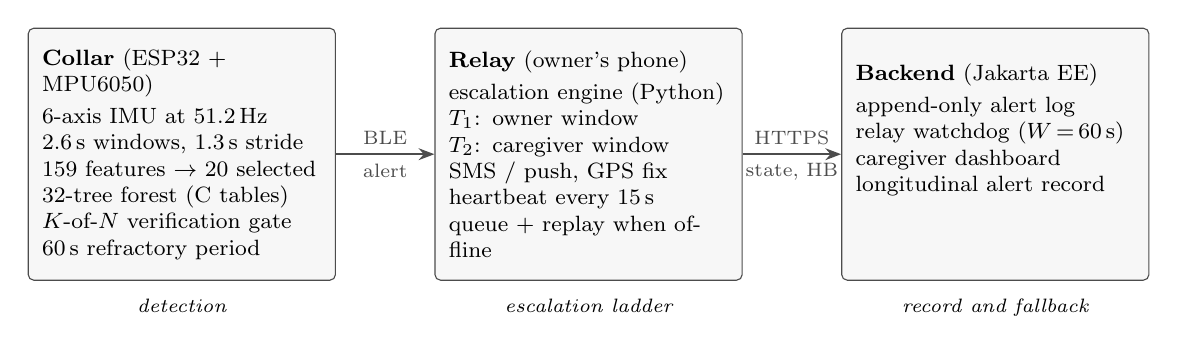
\begin{tikzpicture}[
    font=\footnotesize,
    node/.style={draw=black!70, rounded corners=2pt, fill=black!3, align=left,
                 minimum height=3.2cm, text width=3.55cm, inner sep=5pt},
    head/.style={font=\footnotesize\bfseries},
    link/.style={-{Stealth[length=2mm]}, thick, black!70},
    lab/.style={font=\scriptsize, fill=white, inner sep=1pt}]
  \node[node] (collar) {%
    {\bfseries Collar} (ESP32 + MPU6050)\\[2pt]
    6-axis IMU at 51.2\,Hz\\
    2.6\,s windows, 1.3\,s stride\\
    159 features $\rightarrow$ 20 selected\\
    32-tree forest (C tables)\\
    $K$-of-$N$ verification gate\\
    60\,s refractory period};
  \node[node, right=1.25cm of collar] (relay) {%
    {\bfseries Relay} (owner's phone)\\[2pt]
    escalation engine (Python)\\
    $T_1$: owner window\\
    $T_2$: caregiver window\\
    SMS / push, GPS fix\\
    heartbeat every 15\,s\\
    queue + replay when offline};
  \node[node, right=1.25cm of relay] (backend) {%
    {\bfseries Backend} (Jakarta EE)\\[2pt]
    append-only alert log\\
    relay watchdog ($W$\,=\,60\,s)\\
    caregiver dashboard\\
    longitudinal alert record\\
    \phantom{x}\\
    \phantom{x}};
  \draw[link] (collar) -- node[lab, above=2pt] {BLE} node[lab, below=2pt] {alert} (relay);
  \draw[link] (relay) -- node[lab, above=2pt] {HTTPS} node[lab, below=2pt] {state, HB} (backend);
  \node[below=3pt of collar, font=\scriptsize\itshape] {detection};
  \node[below=3pt of relay, font=\scriptsize\itshape] {escalation ladder};
  \node[below=3pt of backend, font=\scriptsize\itshape] {record and fallback};
\end{tikzpicture}
}
\caption{System architecture. Detection runs on the collar, the escalation ladder on the owner's phone, and the backend keeps the record and acts as a fallback when the phone goes silent.\label{fig:arch}}
\end{figure}

\subsection{Dataset}
\label{sec:data}
We use the public release accompanying Brady et al.~\cite{brady2025collar,song2025figshare}: \R{ds.files}~recordings from \R{ds.sessions}~collection sessions and two Shimmer3 units, \R{ds.seconds}\,s (\R{ds.minutes}\,min) of motion with \R{ds.spins}~annotated spin alerts totalling \R{ds.spinseconds}\,s. Six trained dogs (two Golden Retrievers, two Labradors, two Standard Poodles, aged 1.5--2 years) performed a cued double clockwise spin in training sessions; annotation was against synchronised video~\cite{brady2025collar}. We use the low-noise accelerometer and the gyroscope, the channels our collar's MPU6050 also provides.

Two properties of the release shape the analysis. First, the timestamps give a sampling rate of \R{ds.fs}\,Hz (the Shimmer3's 1024/20 divider), not the 50\,Hz used in the source paper; our spin durations (\R{ds.durmin}--\R{ds.durmax}\,s, median \R{ds.durmedian}\,s) are uniformly 2.4\% shorter than the published ones, exactly the ratio 50/51.2, so we derive all window lengths in samples from the measured rate. Second, the release does not identify the dog in each recording. A literal leave-one-dog-out (LODO) split cannot be reproduced, so we hold out \emph{recording groups} (\R{ds.groups}~groups, \R{ds.eventgroups}~of which yield curated events). A recording group never splits a behavioural episode or a recording across folds, but two recordings of the same dog may fall in different folds; our cross-subject estimates may therefore be optimistic relative to LODO, and we add session- and device-level protocols (Section~\ref{sec:protocols}) partly to bound this.

The gyroscope saturates: \R{sr.gyrosatspin}\% of spin samples and \R{sr.gyrosatnonspin}\% of non-spin samples have at least one axis at the \R{sr.gyrofs}\,\textdegree{}/s full-scale limit. A collar configured for a wider range would see values the training distribution never contained; Section~\ref{sec:robust} examines the consequences.

\subsection{Detection Pipeline}
\label{sec:pipeline}
We re-implement the pipeline of~\cite{brady2025collar}. Signals are cut into \R{cfg.window}\,s windows (\R{cfg.winsamples}~samples) with a \R{cfg.stride}\,s stride (\R{cfg.stridesamples}~samples); a window is labelled \emph{spin} if at least half its samples are annotated spin. For the curated-event protocol each annotated spin is centred in a \R{cfg.eventseconds}\,s event (\R{cfg.eventsamples}~samples, exactly five windows), and spin-free spans at least 1\,s from any spin are tiled into negative events, giving \R{ds.events}~events (\R{ds.posevents}~positive) and \R{ds.windows}~windows (\R{ds.poswindows}~positive).

From the six channels we derive eight signals (the three axes of each sensor and the rotation-invariant magnitudes $|a|$ and $|g|$) and compute 13 time-domain and 5 frequency-domain statistics per signal plus the 15 pairwise channel correlations: \R{cfg.nfeat}~features. A three-stage selector (variance filter, pruning of pairs with $|r|>0.95$, ANOVA $F$-test) keeps \R{cfg.nsel}. Selection, scaling and fitting all happen inside each training fold.

We evaluate the four classifiers of the source study---random forest (RF, 200 trees, depth 12), RBF support-vector machine, Gaussian naive Bayes and logistic regression---and the heuristic baseline (a threshold on mean $|g|$, tuned on the training fold). The model the collar ships is a smaller forest (32 trees, depth 8, \R{fw.kib}\,KiB of flash tables), and every gate and stream result below refers to it unless stated otherwise. As additional baselines on raw windows we evaluate a three-block 1-D CNN (\R{abl.cnnparams} parameters) and ROCKET with 2000 random kernels and a ridge classifier~\cite{dempster2020rocket}, plus histogram gradient boosting on the features.

\subsection{Streaming Verification Gate}
\label{sec:gate}
A single window classified as spin is not an alert. Every stride the gate receives the window's probability $p_t$, records the vote $v_t = \mathbf{1}[p_t \geq \theta]$, and fires when
\begin{equation}
\sum_{i=t-N+1}^{t} v_i \;\geq\; K \quad\text{and}\quad t - t_{\text{last}} \geq R,
\label{eq:gate}
\end{equation}
where $t_{\text{last}}$ is the previous alert and $R=\R{cfg.refractory}$\,s is a refractory period. On firing, the vote buffer is cleared, so that one episode cannot re-fire on stale evidence when the refractory period ends. The alert's confidence is the mean probability of the voting windows. The policy $(\theta,K,N)$ is searched over $\theta \in \{0.25,0.30,\dots,0.50\}$ and nine $(K,N)$ pairs with $1\leq K\leq N\leq 5$, choosing the policy that maximises event sensitivity subject to a per-event false-alarm rate of at most \R{cfg.maxfar}\%, ties broken by fewer false alarms and then lower latency. Because a missed alert and a spurious one have asymmetric costs (a spurious one costs the owner a dismissal), we do not optimise F1.

\subsection{Evaluation Protocols}
\label{sec:protocols}

\textbf{Segment and event level.} Following~\cite{brady2025collar}, we report window-level (segment) metrics and event-level metrics in which a curated event counts as detected if any of its windows is positive. Under leave-one-group-out (LOGO) all out-of-fold predictions are pooled.

\textbf{Shift protocols.} Leave-one-session-out holds out each of the three collection sessions (different days), and leave-one-device-out holds out each Shimmer unit (one session used a different unit), giving temporal- and device-shift estimates with exactly the same fitting code.

\textbf{Nested selection of the gate.} Selecting $(\theta,K,N)$ on the same out-of-fold scores that are then reported biases the reported sensitivity upward~\cite{varma2006bias,cawley2010overfitting}. In the nested protocol, for each held-out group $g$ an inner LOGO over the remaining groups produces out-of-fold scores, the policy is selected on those, and the model refitted on all remaining groups is applied with that policy to $g$. Nothing about $g$ influences the policy applied to it.

\textbf{Continuous streams.} The curated protocol never asks the question a deployed collar faces: \emph{when} does an alert exist in an unbroken stream? We therefore replay every recording end to end---windows every stride, scored by the fold model that never saw the recording's group, through the gate of Equation~(\ref{eq:gate}) with its nested policy. We score alerts with the any-overlap convention of seizure-detection evaluation~\cite{shah2021metrics,dan2025szcore}: an alert at time $t$ is a true detection of a spin $[t_{\text{on}}, t_{\text{off}}]$ if the window that completed the vote overlaps it,
\begin{equation}
t_{\text{on}} \;\leq\; t \;\leq\; t_{\text{off}} + W_{\text{win}} + \tau,
\label{eq:overlap}
\end{equation}
where $W_{\text{win}}$ is the window length and $\tau\geq 0$ an optional post-event tolerance (default 0); every other alert is a false alarm. The false-alarm rate is normalised by \emph{spin-free exposure}, the stream time outside the union of the intervals in Equation~(\ref{eq:overlap}). Spins closer together than $R$ are merged into one \emph{alert episode}, the unit the gate is designed to report once; we report per-spin sensitivity with $R=0$ and per-episode sensitivity with $R=\R{cfg.refractory}$\,s. The streams total \R{ds.hours}\,h; we report $\tau$ as a sensitivity analysis because alerts a few seconds after a spin are behaviourally part of the episode.

\textbf{Uncertainty and tests.} Windows within a recording are strongly dependent, so every interval resamples whole recording groups (cluster percentile bootstrap~\cite{field2007clustered,efron1993bootstrap}, \R{stat.nboot}~resamples). False-alarm rates additionally carry exact Garwood Poisson intervals~\cite{garwood1936} and proportions Wilson score intervals~\cite{wilson1927}. Models are compared against the deployed forest with paired cluster-bootstrap differences in F1 and AUC (Holm-adjusted~\cite{holm1979}), Wilcoxon signed-rank tests on per-fold F1~\cite{wilcoxon1945}, and exact McNemar tests on event-level correctness~\cite{dietterich1998tests}.

\subsection{Escalation Protocol}
\label{sec:ladder}
When the gate fires the relay opens an alert in \textsc{PendingOwner} and notifies the owner locally (Figure~\ref{fig:sm}). If the owner neither acknowledges nor dismisses within $T_1=\R{esc.t1}$\,s, the caregiver is paged and the alert moves to \textsc{PendingCaregiver}; if the caregiver does not acknowledge within a further $T_2=\R{esc.t2}$\,s, the emergency contact is paged. The emergency contact should be a named person or an accredited monitoring service, not an automated call to emergency services. Design commitments, each enforced by tests, are: deadlines are evaluated on an injected monotonic clock (a wall clock can jump); each channel is paged at most once per alert; ingestion is idempotent, because an alert's identity is derived from the collar's episode rather than from arrival time and BLE delivery is at-least-once; a channel that cannot be reached does not stall the ladder; terminal states absorb, so a late acknowledgement is recorded but does not withdraw an escalation; and stale location fixes are dropped rather than sent. While an alert is open the relay heartbeats to the backend every \R{esc.hb}\,s; the backend watchdog, as built, pages the emergency contact directly if the relay is silent for more than $W=\R{esc.w}$\,s.

\begin{figure}[H]
\centering
\resizebox{\linewidth}{!}{% The escalation ladder (relay) with the backend watchdog's take-over edges.
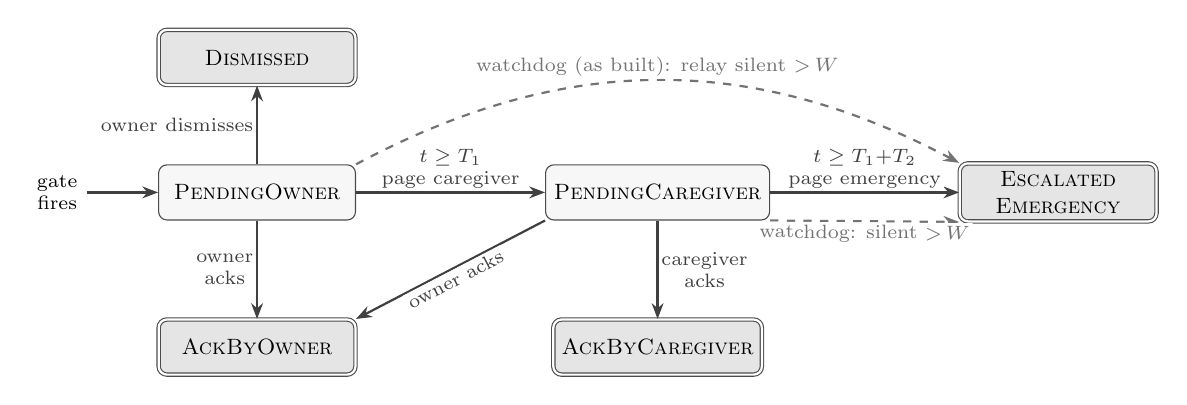
\begin{tikzpicture}[
    font=\footnotesize, >={Stealth[length=2mm]},
    st/.style={draw=black!70, rounded corners=3pt, fill=black!3, minimum height=7mm,
               minimum width=2.5cm, align=center, inner sep=3pt},
    term/.style={st, fill=black!10, double, double distance=0.8pt},
    edge/.style={->, thick, black!75},
    wd/.style={->, thick, dashed, black!55},
    lab/.style={font=\scriptsize, align=center, fill=white, inner sep=1pt}]
  \node[st]   (po) {\textsc{PendingOwner}};
  \node[st,   right=2.4cm of po] (pc) {\textsc{PendingCaregiver}};
  \node[term, right=2.4cm of pc] (em) {\textsc{Escalated}\\\textsc{Emergency}};
  \node[term, below=1.25cm of po] (ao) {\textsc{AckByOwner}};
  \node[term, below=1.25cm of pc] (ac) {\textsc{AckByCaregiver}};
  \node[term, above=1.0cm of po] (di) {\textsc{Dismissed}};
  \node[left=0.9cm of po, font=\scriptsize, align=center] (start) {gate\\fires};
  \draw[edge] (start) -- (po);
  \draw[edge] (po) -- node[lab, above] {$t \geq T_1$\\page caregiver} (pc);
  \draw[edge] (pc) -- node[lab, above] {$t \geq T_1{+}T_2$\\page emergency} (em);
  \draw[edge] (po) -- node[lab, left] {owner\\acks} (ao);
  \draw[edge] (pc) -- node[lab, right] {caregiver\\acks} (ac);
  \draw[edge] (pc.south west) -- node[lab, sloped, below] {owner acks} (ao.north east);
  \draw[edge] (po) -- node[lab, left] {owner dismisses} (di);
  \draw[wd] (po.north east) to[bend left=28] node[lab, above] {watchdog (as built): relay silent ${>}\,W$} (em.north west);
  \draw[wd] (pc.south east) to[bend right=0] node[lab, sloped, below] {watchdog: silent ${>}\,W$} (em.south west);
\end{tikzpicture}
}
\caption{The escalation ladder run by the relay (solid) and the backend watchdog's take-over edges as built (dashed). Double borders mark terminal states. Section~\ref{sec:formal-results} shows why the dashed edge from \textsc{PendingOwner} is a design flaw and gives the ladder-aware replacement.\label{fig:sm}}
\end{figure}

\subsection{Formal Model and Conformance Testing}
\label{sec:formal}
We specify one alert episode in TLA$^+$~\cite{lamport2002specifying} (file S1): the relay's ladder, the owner and caregiver (who may respond at any moment, or never), per-episode caregiver reachability, a network between relay and backend that may partition and heal at any time, a relay that may die, heartbeats, transition mirroring with an offline queue, and the watchdog. Time is discrete with one tick per heartbeat interval, so $T_1$, $T_2$ and $W$ are \R{tlc.t1}, \R{tlc.t2} and \R{tlc.w} ticks; ticks are \emph{urgent}---time cannot pass while a timer, heartbeat or watchdog sweep is due---which models drivers that run at least once per tick. The check is bounded at \R{tlc.horizon}~ticks, beyond the latest possible escalation. A constant selects the watchdog variant: \emph{Direct} (as built) or \emph{Ladder}, which on relay silence continues the ladder on the relay's behalf---paging the caregiver once $T_1$ has elapsed and the emergency contact once $T_1+T_2$ has elapsed, both measured from the alert. Each property is checked in its own TLC run~\cite{yu1999tlc} so that one violation cannot mask another, and reachability witnesses (properties that \emph{must} fail) guard against vacuous passes.

To connect the model to the code, property-based tests~\cite{maciver2019hypothesis} drive the shipped engine with random interleavings of clock advances, ticks, acknowledgements, dismissals, cancellations and duplicate submissions, under random policies and delivery failures, checking the model's invariants after every step (\R{prop.examples}~examples per property).

\subsection{End-to-End Monte-Carlo Simulation}
\label{sec:sim}
Model checking says which outcomes are possible; it does not say how likely they are. We simulate genuine alert episodes in one-second steps (the relay's tick rate) with the \emph{real} escalation engine and a port of the watchdog. Each episode samples: whether the collar detects the alert (probability equal to the measured nested continuous-stream episode sensitivity) and its latency (drawn from the measured latencies); optionally, up to $M$ repetitions of the alert 30\,s apart if it goes undetected; the owner's response (whether, and a log-normal delay); the caregiver's availability and delay; per-page delivery loss; and, in stress scenarios, relay death or a network partition at a uniformly random time in the first 240\,s. All human parameters are \emph{assumptions} (Table~\ref{tab:assumptions}), and we report a sensitivity analysis over them. Each scenario uses \R{sim.n}~episodes.

\begin{table}[H]
\caption{Behavioural assumptions of the simulation. Response delays are log-normal with the given median and log-scale $\sigma$. These are not measurements; Section~\ref{sec:sim-results} varies them.\label{tab:assumptions}}
\begin{tabularx}{\textwidth}{lCCC}
\toprule
\textbf{Party} & \textbf{P(responds)} & \textbf{Median delay (s)} & $\boldsymbol{\sigma}$\\
\midrule
Owner, awake & \R{asm.awake.p} & \R{asm.awake.med} & \R{asm.awake.sig}\\
Owner, asleep & \R{asm.asleep.p} & \R{asm.asleep.med} & \R{asm.asleep.sig}\\
Owner, incapacitated & 0 & --- & ---\\
Caregiver & \R{asm.care.p} & \R{asm.care.med} & \R{asm.care.sig}\\
Emergency contact (monitoring service) & \R{asm.emerg.p} & \R{asm.emerg.med} & \R{asm.emerg.sig}\\
\midrule
Page delivery loss (each page) & \multicolumn{3}{c}{\R{asm.loss}}\\
\bottomrule
\end{tabularx}
\end{table}

\textbf{False-alarm burden.} A false alarm reaches the caregiver only if the owner does not dismiss it within $T_1$, and the emergency tier only if the caregiver then does not answer within $T_2$. With a false-alarm rate $\lambda$ (per hour of wear), $h_w$ waking and $h_s$ sleeping hours per day and owner response CDFs $F_w$, $F_s$, the expected caregiver pages per day are
\begin{equation}
C(\lambda) \;=\; \lambda \left[\, h_w \bigl(1 - F_w(T_1)\bigr) + h_s \bigl(1 - F_s(T_1)\bigr) \right],
\label{eq:burden}
\end{equation}
and emergency pages per day are $C(\lambda)\,[1-(1-\ell)F_c(T_2)]$, with $F_c$ the caregiver CDF and $\ell$ the page-loss probability. We assume the owner dismisses a false alarm on the same delay distribution with which they would acknowledge a real one, and $h_w=16$, $h_s=8$. Equation~(\ref{eq:burden}) is checked against the simulation in the test suite. Inverting it for a target of one caregiver page per week gives the largest tolerable $\lambda$.

\subsection{Embedded Implementation and Sensor Transfer}
\label{sec:embedded}
The collar's algorithmic core (features, forest walk, gate, sample ring) is portable C99 with no Arduino dependency, so it compiles on a host and is tested against golden vectors produced by the Python pipeline from real dataset windows. The fitted forest is transpiled to flat integer and float tables; the exporter refuses to write a model whose transpiled predictions differ from scikit-learn's by more than $10^{-6}$. Variances use a two-pass computation: the one-pass form loses too much precision in float32 on a gyroscope channel. The frequency features use a direct 133-point DFT, because zero-padding to a power of two for an FFT would change the spectrum the model was trained on; the DFT reads a precomputed twiddle table rather than calling \texttt{sinf}/\texttt{cosf} in the inner loop. We measure per-window cost on the host and report machine-independent operation counts.

To study transfer to the MPU6050~\cite{invensense2013mpu6000} without hardware, we perturb held-out windows only, with models trained on clean data, using: rigid collar rotations about each device axis and uniformly random rotations in SO(3); the datasheet's noise densities, zero-rate and zero-$g$ offsets and sensitivity tolerances; clipping and 16-bit quantisation at the configured full scale; a narrower gyroscope full scale; sampling jitter; and sampling-rate mismatch. We repeat the rotations with a model trained on rotation-augmented data~\cite{um2017augmentation} and with a model restricted to the rotation-invariant magnitude features.

\subsection{Software and Reproducibility}
All analyses use Python with NumPy, SciPy, scikit-learn and PyTorch~\cite{harris2020numpy,virtanen2020scipy,pedregosa2011sklearn,paszke2019pytorch}; the escalation layer and the simulation use only the Python standard library. A single command regenerates every artifact, figure and number in this paper; fixed seeds are used throughout.

\textbf{Use of generative AI.} A large language model (Claude, Anthropic) was used to assist with implementing the analysis software, the TLA$^+$ specification and the simulation, with verifying bibliographic metadata, and with drafting the manuscript. It was not used to generate or alter data. All analyses run from the released code on the public dataset, every reported number is regenerated from that code (Appendix~\ref{app:repro}), every reference was checked against its DOI, and the authors reviewed and take responsibility for all content.

\section{Results}
\label{sec:results}

\subsection{Detection: Reproduction and Uncertainty}
\label{sec:res-detection}
Table~\ref{tab:logo} and Figure~\ref{fig:models} report the detection layer under LOGO. The supervised models beat the heuristic at segment level: the heuristic's F1 is lower than the deployed forest's by \R{cmp.base.dF1} (95\% cluster-bootstrap interval of the difference \R{cmp.base.dF1CI}, Holm-adjusted $p=\R{cmp.base.pF1}$)---and at event level the deployed forest is correct on \R{cmp.base.mcB} events on which the heuristic is wrong against \R{cmp.base.mcC} the other way (exact McNemar $p=\R{cmp.base.mcP}$). The heuristic's AUC, however, is not distinguishable from the forest's (difference \R{cmp.base.dAUC}, \R{cmp.base.dAUCCI}): a single mean-gyroscope-magnitude statistic ranks windows almost as well as 20 selected features, and the learned models' advantage is in calibrating a decision boundary rather than in separating the classes. Among the learned models no difference from the deployed 32-tree forest survives correction, including the 200-tree reference forest (F1 difference \R{cmp.rf.dF1CI}) and the SVM (\R{cmp.svm.dF1CI}). Within-subject F1 (random split, optimistic by construction) exceeds LOGO F1 for every model, reproducing the source study's observation that cross-subject difficulty lies in the minority class.

The intervals are wide. The deployed forest's event recall is \R{logo.rfe.evRec} with a 95\% interval of \R{logo.rfe.evRecCI}; with \R{ds.eventgroups}~groups, of which a handful contribute most of the spins, the data cannot pin the detector down to better than about $\pm0.1$ in recall, and point estimates that differ by a few hundredths should not be ranked.

\begin{table}[H]
\caption{Detection under leave-one-group-out. Bracketed values are 95\% cluster-bootstrap intervals over recording groups. Within-subject F1 uses a random window split and is optimistic by construction. Raw-window baselines and gradient boosting share the same folds.\label{tab:logo}}
\begin{adjustwidth}{-\extralength}{0cm}
\small
\begin{tabularx}{\fulllength}{lccccc}
\toprule
\textbf{Model} & \textbf{Within F1} & \textbf{LOGO segment F1} & \textbf{LOGO segment AUC} & \textbf{Event recall} & \textbf{Event specificity}\\
\midrule
\inputtable{generated/tables/logo.tex}
\bottomrule
\end{tabularx}
\end{adjustwidth}
\end{table}

\begin{figure}[H]
\centering
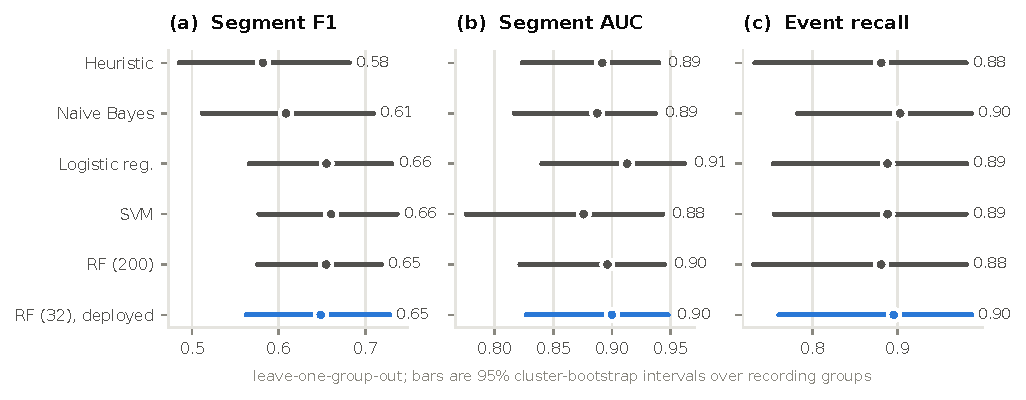
\includegraphics[width=\linewidth]{figures/fig_models.pdf}
\caption{Detection metrics under LOGO with 95\% cluster-bootstrap intervals. The deployed forest is highlighted. Intervals overlap for all learned models.\label{fig:models}}
\end{figure}

\textbf{Learned features do not help on this dataset.} Neither raw-window model beats the hand-crafted pipeline: ROCKET reaches segment F1 \R{abl.rocket.F1} (AUC \R{abl.rocket.AUC}) and the 1-D CNN \R{abl.cnn.F1} (AUC \R{abl.cnn.AUC}), against \R{abl.rfe.F1} (AUC \R{abl.rfe.AUC}) for the deployed forest; gradient boosting on the features is comparable to the forest (\R{abl.hgb.F1}, AUC \R{abl.hgb.AUC}). With \R{ds.poswindows}~positive windows, a model that must learn its own features has little to learn from.

\textbf{Ablations.} The rotation-invariant magnitude features alone (\R{fam.magnitudesonly.n} features) reach segment F1 \R{fam.magnitudesonly.F1} and AUC \R{fam.magnitudesonly.AUC}, and the \R{fam.gyromagnitudeonly.n} gyroscope-magnitude features alone reach \R{fam.gyromagnitudeonly.F1} and \R{fam.gyromagnitudeonly.AUC}---no worse than all \R{cfg.nfeat}. Accelerometer-only features are clearly weaker (F1 \R{fam.accelonly.F1}). A 2.1\,s window scored higher than the source study's 2.6\,s (F1 \R{win.2p1.F1} vs.\ \R{win.2p6.F1}) and longer windows were worse (3.6\,s: \R{win.3p6.F1}). These comparisons were made on the same LOGO folds that they are reported on and are hypothesis-generating; we did not change the shipped configuration on the strength of them, but they matter for Section~\ref{sec:robust}.

\textbf{Shift protocols.} Holding out a whole collection session or a whole Shimmer unit (Table~\ref{tab:shift}) leaves segment AUC essentially unchanged (deployed forest: \R{loso.rfe.segAUC} and \R{lodo.rfe.segAUC}, against \R{logo.rfe.segAUC} under LOGO) but moves event recall and specificity by several points in both directions. The heuristic keeps its recall under shift at the cost of much lower specificity (\R{loso.base.evSpec} under leave-one-session-out). Training on one Shimmer unit and testing on the other is the closest proxy the data offer for a change of hardware, and it costs the deployed forest event recall (\R{lodo.rfe.evRec} vs.\ \R{logo.rfe.evRec}).

\begin{table}[H]
\caption{Session and device shift. Leave-one-session-out holds out each of the three collection days; leave-one-device-out holds out each Shimmer3 unit.\label{tab:shift}}
\begin{adjustwidth}{-\extralength}{0cm}
\small
\begin{tabularx}{\fulllength}{lCCCCCCCC}
\toprule
 & \multicolumn{4}{c}{\textbf{Leave-one-session-out}} & \multicolumn{4}{c}{\textbf{Leave-one-device-out}}\\
\cmidrule(lr){2-5}\cmidrule(lr){6-9}
\textbf{Model} & \textbf{F1} & \textbf{AUC} & \textbf{Ev.\ rec.} & \textbf{Ev.\ spec.} & \textbf{F1} & \textbf{AUC} & \textbf{Ev.\ rec.} & \textbf{Ev.\ spec.}\\
\midrule
\inputtable{generated/tables/shift.tex}
\bottomrule
\end{tabularx}
\end{adjustwidth}
\end{table}

\subsection{The Verification Gate and Continuous Streams}
\label{sec:res-gate}
On curated events, the single-level sweep over \R{sweep.npolicies}~policies selects \R{single.rfe.policy} for the deployed forest, with event sensitivity \R{op.single.sens} and \R{op.single.far}\% false alarms per negative event (Figure~\ref{fig:gate}a). Requiring three votes caps sensitivity (best \R{sweep.bestsens.k3} at $K=3$ against \R{sweep.bestsens.k2} at $K=2$): the trained alert lasts about 2.5\,s, a window 2.6\,s, and at a 1.3\,s stride only two or three windows can be majority-spin.

\textbf{Nested selection.} Under nested selection the procedure chose \R{nest.rfe.npolicies} different policies across the \R{nest.rfe.nfolds}~outer folds (most often \R{nest.rfe.modal}, in \R{nest.rfe.modalcount} folds). Its out-of-sample event sensitivity is \R{nest.rfe.sens} (\R{nest.rfe.sensCI}) at \R{nest.rfe.far}\% (\R{nest.rfe.farCI}\%) false alarms per negative event, which slightly exceeds the 5\% bound the policy was selected to meet. Single-level selection was not optimistic here---the nested estimate is \R{nest.rfe.absdiff} \emph{higher} than the single-level one, well inside its interval---and the main thing nesting reveals is how unstable the selected policy is: with this little data, which policy wins depends on which recording is held out.

\textbf{Continuous streams.} Table~\ref{tab:streams} and Figure~\ref{fig:gate}b give the result that most changes the picture. Replaying whole recordings with held-out models and the nested policy, strict any-overlap scoring and no refractory period gives \R{cont.rfe.r0.fah}~FA/h (95\% exact interval \R{cont.rfe.r0.fahCI}) over \R{cont.rfe.r0.exposure}\,h of spin-free exposure---\R{cont.ratio.curated}$\times$ the \R{op.single.fah}~FA/h that the curated-event protocol implies for the same detector. The curated protocol omits exactly the motion where false alarms concentrate: its negative events are kept at least 1\,s from any spin and must fit whole between spins, so the approach to, and recovery from, a spin are never scored. Allowing a post-spin tolerance shows how much of the excess is boundary timing (Figure~\ref{fig:gate}b): with $\tau=10$\,s the rate falls to \R{cont.rfe.tol10.fah}~FA/h and with $\tau=20$\,s to \R{cont.rfe.tol20.fah}~FA/h---still roughly twice the curated estimate, so most of the gap is not a scoring artefact. With the 60\,s refractory period, \R{cont.rfe.r60.epdet} of \R{cont.rfe.r60.epn} alert episodes are detected (\R{cont.rfe.r60.epsens}, \R{cont.rfe.r60.epsensCI}) at \R{cont.rfe.r60.fah}~FA/h, with a median latency of \R{cont.rfe.r60.lat}\,s from the dog starting to spin.

On continuous streams the learned models' advantage largely disappears. The heuristic, also with a nested policy, detects \R{cont.base.r60.epsens} of episodes at \R{cont.base.r60.fah}~FA/h with the refractory period---indistinguishable from the forest at this sample size---although without the refractory period its false-alarm rate (\R{cont.base.r0.fah}~FA/h) is substantially higher than the forest's.

\begin{figure}[H]
\centering
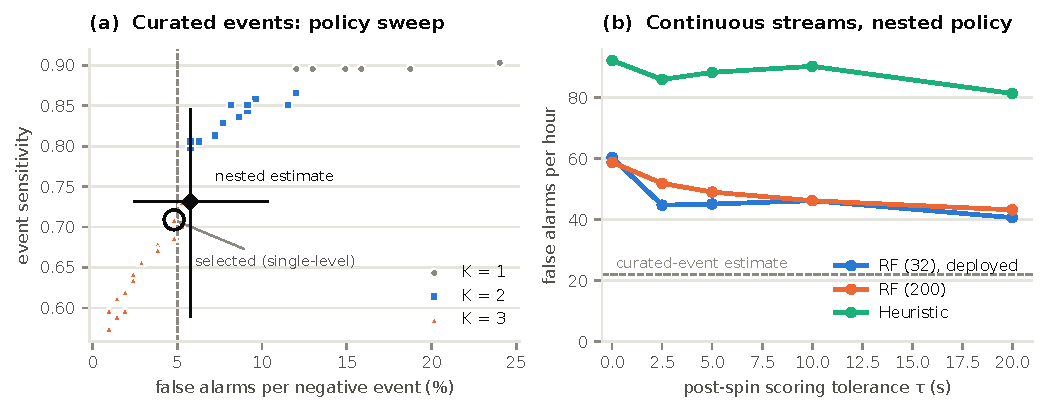
\includegraphics[width=\linewidth]{figures/fig_gate.pdf}
\caption{(\textbf{a}) The $K$-of-$N$ policy sweep on curated events for the deployed forest; the ring marks the single-level selection and the diamond the nested out-of-sample estimate with 95\% intervals. (\textbf{b}) False alarms per hour on continuous recordings as a function of the post-spin scoring tolerance $\tau$ (no refractory period, nested policy); the dashed line is the rate the curated protocol implies.\label{fig:gate}}
\end{figure}

\begin{table}[H]
\caption{Gate performance with nested policy selection: on curated events, and on continuous recordings with strict any-overlap scoring ($\tau=0$). Without the refractory period ($R=0$) every spin is a target; with $R=60$\,s spins closer than 60\,s form one episode. Intervals on FA/h are exact Poisson.\label{tab:streams}}
\begin{adjustwidth}{-\extralength}{0cm}
\small
\footnotesize
\begin{tabular}{lccccccc}
\toprule
 & \multicolumn{2}{c}{\textbf{Curated events}} & \multicolumn{2}{c}{\textbf{Stream, $R=0$}} & \multicolumn{3}{c}{\textbf{Stream, $R=60$\,s}}\\
\cmidrule(lr){2-3}\cmidrule(lr){4-5}\cmidrule(lr){6-8}
\textbf{Model} & \textbf{Sens.} & \textbf{FA/ev.\ (\%)} & \textbf{Spin sens.} & \textbf{FA/h} & \textbf{Ep.\ sens.} & \textbf{FA/h} & \textbf{Lat.\ (s)}\\
\midrule
\inputtable{generated/tables/streams.tex}
\bottomrule
\end{tabular}
\end{adjustwidth}
\end{table}

Figure~\ref{fig:timeline} shows one held-out recording end to end.

\begin{figure}[H]
\centering
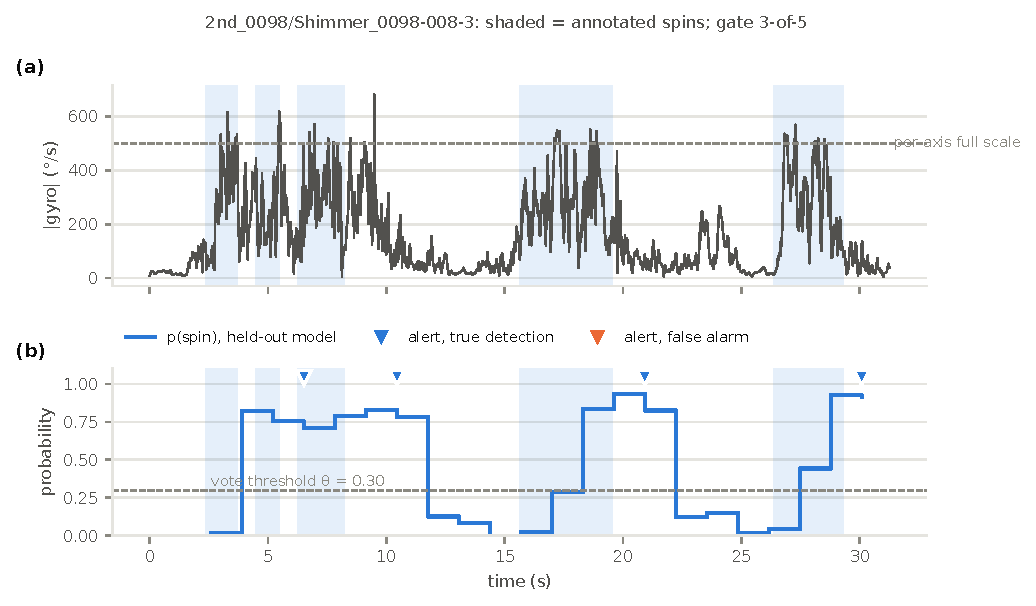
\includegraphics[width=\linewidth]{figures/fig_timeline.pdf}
\caption{One held-out recording (\TimelineRecording) as the collar would process it. (\textbf{a}) Gyroscope magnitude; shaded spans are annotated spins; the dashed line is the per-axis full scale at which the Shimmer3 saturates. (\textbf{b}) Window probabilities from a model that never saw this recording's group, the vote threshold, and the alerts the gate raises (refractory period off for visibility).\label{fig:timeline}}
\end{figure}

\subsection{Formal Verification of the Escalation Protocol}
\label{sec:formal-results}
Table~\ref{tab:tlc} lists the \R{tlc.nchecks} TLC checks (\R{tlc.nwitness} of which are reachability witnesses, omitted from the table, all violated as required). Every check came out as expected. For the system as built, every safety property of the ladder itself holds under arbitrary owner and caregiver behaviour, relay death and network partitions: no channel is paged twice; the relay pages the emergency contact only after $T_1+T_2$ (or $T_1$ with no caregiver configured); the relay never escalates after the owner responded; with a live relay every alert closes by $T_1+T_2$; if the backend ever learned of the alert, it closes within $T_1+T_2+W+1$ ticks even if the relay dies; and terminal states absorb. With a reliable phone and network, the three end-to-end properties also hold.

Under faults, TLC produced counterexamples to three properties, each of which is a real behaviour of the design:

\begin{enumerate}
\item \textbf{The watchdog skips the caregiver tier.} In the shortest counterexample (Appendix~\ref{app:cex}) the phone dies one tick after mirroring the alert. The backend sees an open alert and no heartbeats, and the Direct watchdog pages the emergency contact at tick \R{tlc.premature.tick} (\R{tlc.premature.s}\,s)---before the caregiver would have been paged at $T_1$---and, the phone being dead, the caregiver is never paged at all. A network partition produces the same premature page while the relay is still alive; the relay then escalates on its own as well, and the emergency contact is paged twice (the \texttt{AtMostOneEmergencyPage} counterexample).
\item \textbf{A lost acknowledgement causes an emergency page.} The owner acknowledges; the phone dies before mirroring that to the backend; the watchdog sees an open alert with a silent relay and escalates. This is the designed ``err towards escalating'' behaviour, and model checking makes its cost explicit.
\item \textbf{An alert can be lost silently.} If the network is down when the gate fires and the phone dies before it reconnects, the backend never learns of the alert and nobody beyond the owner's dead phone is ever told. No backend design can repair this; only a second path from the collar can.
\end{enumerate}

The \emph{Ladder} watchdog removes the first defect. It is verified never to page the emergency contact before $T_1+T_2$, preserves at-most-once paging by each party and the bounded-response guarantee, and can still reach the emergency contact; duplicate pages between relay and backend under a partition remain possible and require idempotent paging at a shared provider.

\begin{table}[H]
\caption{TLC results (reachability witnesses omitted). ``Reliable'': phone never dies and network never partitions; ``faults'': both may happen at any time. Direct: watchdog as built; Ladder: proposed variant.\label{tab:tlc}}
\small
\begin{tabularx}{\textwidth}{>{\raggedright\arraybackslash}Xlllr}
\toprule
\textbf{Property} & \textbf{Model} & \textbf{Watchdog} & \textbf{Verdict} & \textbf{States}\\
\midrule
\inputtable{generated/tables/tlc.tex}
\bottomrule
\end{tabularx}
\end{table}

\textbf{Conformance and an integration defect.} The property-based tests found no disagreement between the shipped engine and the model's invariants in \R{prop.examples}~random executions per property. Writing the model, however, required stating precisely how the backend associates heartbeats with alerts---and the code did it inconsistently: the relay labelled heartbeats with the \emph{owner's} contact identifier while the watchdog matched them against the alert's \emph{dog} identifier. The two never matched, so in deployment the watchdog would have treated every relay as one that had never heartbeated and would have fallen back to its 600\,s ceiling. Every unit test passed with the bug present, because each side was tested against its own fixtures. We fixed it and added a regression test.

\subsection{End-to-End Outcomes}
\label{sec:sim-results}
With the measured detector (episode sensitivity \R{sim.pdetect}), the dominant loss in every scenario is the alert that is never detected (Figure~\ref{fig:sim}a). When the owner is incapacitated, a human responds within 300\,s in \R{sim.ownerincapacitated.p300}\% of episodes (median \R{sim.ownerincapacitated.median}\,s among those reached), and the ladder delivers that response in \R{sim.ownerincapacitated.p300givendet}\% of the episodes the collar detects. If the dog repeats an unacknowledged alert up to three times, 30\,s apart, detection rises to \R{sim.rep3.pdet}\% and the 300\,s figure to \R{sim.rep3.p300}\%, at the cost of a later median (\R{sim.rep3.median}\,s). Whether trained dogs repeat in this way is not in the dataset, and it is the single largest lever on outcomes available without better sensing. When the owner is awake, \R{sim.ownerawake.byowner}\% of episodes are closed by the owner and only \R{sim.ownerawake.care}\% reach the caregiver; asleep, \R{sim.ownerasleep.care}\% do.

Fault injection reproduces the model-checking findings quantitatively (Figure~\ref{fig:sim}b). With the phone dying at a random time in the first 240\,s while the owner is incapacitated, the Direct watchdog skips the caregiver tier in \R{sim.incapacitatedrelaydies.skipped}\% of episodes; the Ladder watchdog in \R{sim.incapacitatedrelaydies.ladder.skipped}\%. Under partitions, duplicate emergency pages occur in \R{sim.incapacitatedpartition.dup}\% of episodes with the Direct watchdog and \R{sim.incapacitatedpartition.ladder.dup}\% with the Ladder watchdog, and with an awake owner \R{sim.awakepartition.afterack}\% of episodes page someone after the owner has already responded. Alerts lost because the phone died before the backend heard of them occur in \R{sim.incapacitatedrelaydies.lost}\% of those stress episodes. The sensitivity analysis over the asleep-owner assumptions is informative mainly about speed. Within 300\,s the monitoring tier catches nearly every detected episode that owner and caregiver miss, so that figure moves only between \R{tornado.p300.min}\% and \R{tornado.p300.max}\% across all variations---it is governed by detection, not by the humans. Within 180\,s it ranges from \R{tornado.p180.min}\% to \R{tornado.p180.max}\%, most strongly with caregiver availability (\R{tornado.care.lo}\% at \R{tornado.care.vlo} to \R{tornado.care.hi}\% at \R{tornado.care.vhi}) and caregiver response time (\R{tornado.caremed.lo}\% at a \R{tornado.caremed.vlo}\,s median to \R{tornado.caremed.hi}\% at \R{tornado.caremed.vhi}\,s).

\begin{figure}[H]
\centering
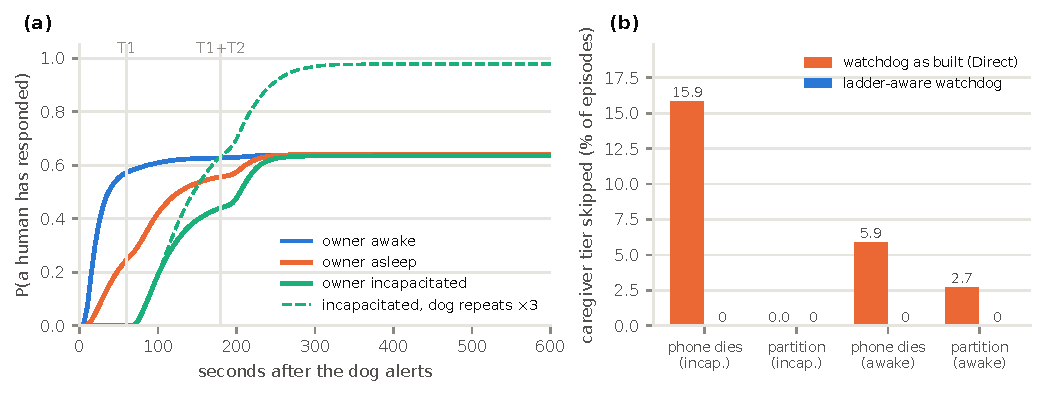
\includegraphics[width=\linewidth]{figures/fig_sim.pdf}
\caption{(\textbf{a}) Probability that a human has responded, by time after the dog alerts, for three owner states and for an incapacitated owner whose dog repeats an unacknowledged alert. The curves plateau below 1 because undetected alerts never start the ladder. (\textbf{b}) Share of episodes in which the emergency contact is paged before any caregiver page, under injected faults, for the watchdog as built and the ladder-aware variant.\label{fig:sim}}
\end{figure}

\textbf{False-alarm burden and the requirement it implies.} With the shipped timings and the assumed owner behaviour, \R{burden.preach}\% of false alarms reach the caregiver: the owner-acknowledgement stage attenuates false alarms by a factor of \R{burden.attenuation} before they reach anyone else. That is not enough. At the measured training-session rate of \R{burden.measured.fah}~FA/h a caregiver would be paged about \R{burden.measured.careday} times a day. Inverting Equation~(\ref{eq:burden}) for one caregiver page per week requires a detector false-alarm rate of at most \R{req.maxfah}~FA/h (\R{req.maxfaday} per day; Figure~\ref{fig:burden}a)---\R{req.factor}$\times$ below the measured rate, and of the same order as the 0.2--2.5 false alarms per day of clinically validated seizure wearables~\cite{naganur2022meta,meritamlarsen2023nonEEG}. One emergency page per month requires \R{req.maxfahemerg}~FA/h. The timing grid (Figure~\ref{fig:burden}b) shows the trade-off the ladder can offer on top of this: shortening $T_1$ to 30\,s raises the probability of help within 180\,s for an incapacitated owner but lets \R{grid.t1short.preach}\% of false alarms through to the caregiver, against \R{burden.preach}\% at 60\,s and \R{grid.t1long.preach}\% at 120\,s.

\begin{figure}[H]
\centering
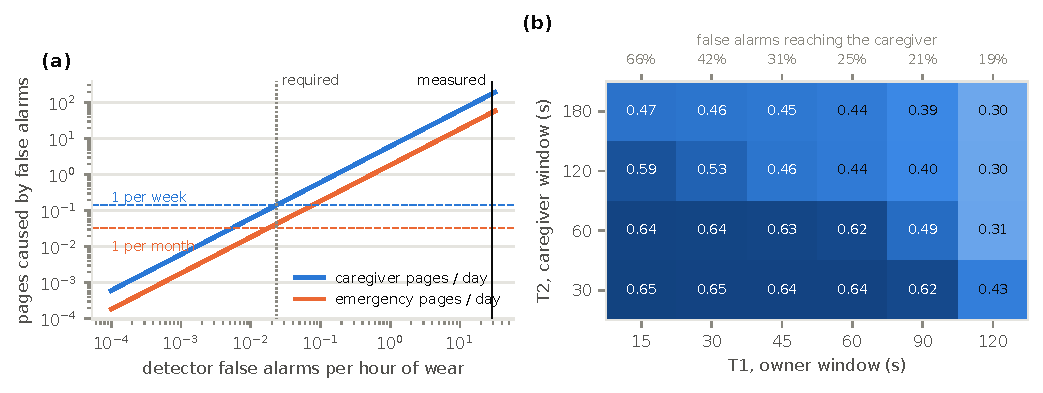
\includegraphics[width=\linewidth]{figures/fig_burden.pdf}
\caption{(\textbf{a}) Pages caused by false alarms alone as a function of the detector's false-alarm rate, with the shipped $T_1=60$\,s and $T_2=120$\,s; the vertical lines mark the measured training-session rate and the rate that keeps caregiver pages to one per week. (\textbf{b}) Probability that a human responds within 180\,s when the owner is incapacitated, over the $(T_1, T_2)$ grid; the top axis gives the share of false alarms that reach the caregiver for each $T_1$.\label{fig:burden}}
\end{figure}

\subsection{Embedded Implementation and Sensor Transfer}
\label{sec:robust}
The transpiled forest (\R{fw.trees}~trees, \R{fw.nodes}~nodes, \R{fw.kib}\,KiB) agrees with scikit-learn to \R{fw.transpile} in probability; the complete C pipeline, from raw window to probability, agrees with the Python pipeline to \R{fw.probaerr} on \R{fw.windows}~real windows, with worst feature relative error \R{fw.featerr}, and passes all \R{fw.checks}~host checks. The size/accuracy front over \R{front.n}~forest configurations (Figure~\ref{fig:front}) is flat: segment AUC spans only \R{front.aucmin}--\R{front.aucmax}, and \R{front.small.trees}~trees of depth \R{front.small.depth} (\R{front.small.kib}\,KiB) come within 0.01 AUC of the shipped forest. On the host, one window costs \R{bench.us}\,$\mu$s with the twiddle-table DFT against \R{bench.direct.us}\,$\mu$s with in-loop \texttt{sinf}/\texttt{cosf} (\R{bench.trig}~transcendental calls per window); the forest walk visits \R{bench.visits}~nodes. We have not measured the cost on an ESP32 and report no estimate of it.

\begin{figure}[H]
\centering
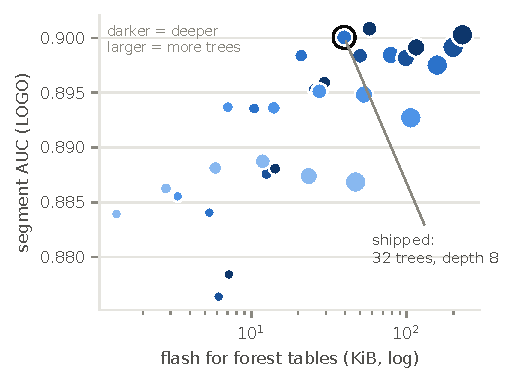
\includegraphics[width=0.62\linewidth]{figures/fig_front.pdf}
\caption{Segment AUC against flash footprint for \R{front.n} forest configurations (4--128 trees, depth 4--12) under LOGO.\label{fig:front}}
\end{figure}

\textbf{Transfer to the MPU6050.} Passing held-out windows through the datasheet's noise, offset and sensitivity errors and 16-bit quantisation leaves event recall unchanged (\R{rob.c.mpu6050datasheet.evRec} vs.\ \R{rob.c.clean.evRec}; Figure~\ref{fig:robust}), as do 5\,ms sampling jitter and a 50\,Hz rather than 51.2\,Hz collar. Range does matter: restricting the gyroscope to a 250\,\textdegree{}/s full scale---the MPU6050's power-on default---drops event recall to \R{rob.c.gyrofullscale250dps.evRec}, whereas the $\pm$2000\,\textdegree{}/s range the firmware configures loses nothing (and a 45\,Hz collar costs little, \R{rob.c.rate45hz.evRec}). \textbf{Collar rotation is the dominant risk.} A 90\textdegree{} rotation about the device $x$ axis drops event recall to \R{rob.c.rotx90deg.evRec}, and about $z$ to \R{rob.c.rotz90deg.evRec}; a uniformly random orientation to \R{rob.c.rotrandomso3.evRec}. Training with two randomly rotated copies of every window restores recall (\R{rob.a.rotrandomso3.evRec} under random rotation) at a small cost on unrotated data (\R{rob.a.clean.evRec}), and the magnitude-only model is invariant by construction: its event recall is \R{rob.m.rotrandomso3.evRec} under every rotation, slightly below the unrotated full model's \R{rob.c.clean.evRec}. Because a collar does rotate around the neck between fittings, we recommend one of the two for any physical deployment.

\begin{figure}[H]
\centering
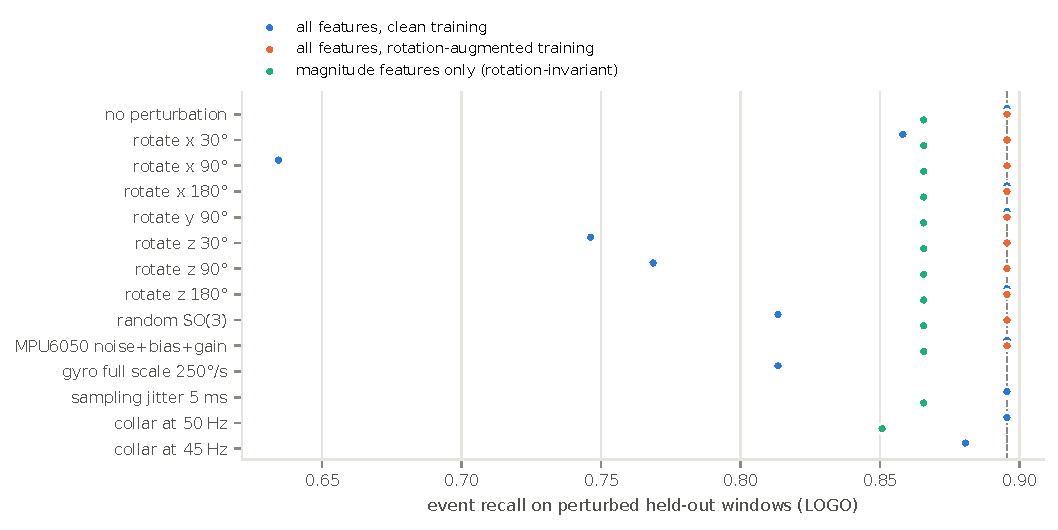
\includegraphics[width=\linewidth]{figures/fig_robustness.pdf}
\caption{Event recall of the deployed configuration on held-out windows under simulated sensor-transfer perturbations, for clean training, rotation-augmented training, and a model restricted to rotation-invariant magnitude features. The dashed line is unperturbed performance.\label{fig:robust}}
\end{figure}

\section{Discussion}
\label{sec:discussion}

\subsection{Principal Findings}
\textbf{Escalation is necessary, and it can be made provably correct---but it cannot repair detection.} When the owner cannot respond, the ladder converts \R{sim.ownerincapacitated.p300givendet}\% of \emph{detected} alerts into a human response within five minutes in simulation, and its safety properties hold in every interleaving the model checker explored. Yet the end-to-end figure (\R{sim.ownerincapacitated.p300}\%) is set almost entirely by the detector's episode sensitivity (\R{sim.pdetect}). Everything downstream of the gate multiplies by that number. The cheapest available improvement is behavioural rather than computational: if the dog repeats an unacknowledged alert, detection rises to \R{sim.rep3.pdet}\% without any change to the model.

\textbf{Measured honestly, the false-alarm rate is far above what any escalation chain tolerates.} The owner-acknowledgement stage does real work: it stops roughly three in four false alarms (\R{burden.preach}\% get through with the shipped $T_1$). The detector, however, produces \R{cont.rfe.r60.fah}~FA/h on continuous training-session motion even with the refractory period, and \R{cont.rfe.r0.fah}~FA/h without it. Our burden analysis turns this into a requirement: \R{req.maxfah}~FA/h for one caregiver page per week, three orders of magnitude below what we measure, and comparable to what clinically validated seizure wearables achieve~\cite{naganur2022meta,meritamlarsen2023nonEEG}. That number, rather than a further increment in F1, is what we propose as the target for detection work in this application. The negatives in this dataset are the hardest available---a dog being actively cued, seconds from spinning on command---so the all-day rate is very probably lower. It is unmeasured, and the source study's 412.6\,h of unlabelled wear data~\cite{brady2025collar} is what would measure it.

\textbf{Curated-clip evaluation understates false alarms.} The protocol inherited from the source study scores fixed clips that keep away from spins, and implies \R{op.single.fah}~FA/h; scoring the same detector on continuous recordings gives \R{cont.ratio.curated}$\times$ that. A large part of the difference survives even generous post-spin tolerances. For any system whose output triggers an action, we recommend that this field adopt what seizure detection already standardised~\cite{dan2025szcore,beniczky2018standards}: continuous-recording, event-based scoring, false alarms normalised by exposure, and operating points chosen out of sample.

\textbf{On this data, learned models add calibration, not discrimination.} A one-statistic heuristic matches the forest's AUC, matches it on continuous streams once a refractory period is applied, and neither a CNN nor ROCKET helps. With 135 events from six dogs this is unsurprising, and it argues for collecting data before engineering models.

\textbf{Formal methods paid for themselves.} A bounded model of a small protocol found a design flaw (the watchdog bypassing the caregiver tier when the phone fails) that the existing unit tests and the end-to-end replay never exercised, and writing the model exposed an integration bug that disabled the watchdog in deployment while every test passed. Both are the kind of defect that surfaces only in an incident review; here they surfaced at design time. The heartbeat fix and its regression test are now part of the system; the Ladder watchdog is specified, model-checked and simulated, and porting it to the production backend is listed under future work. We suggest that any alerting system that splits its state across a device and a server is worth the same treatment.

\subsection{Relation to the Source Study}
Our LOGO segment F1 for the 200-tree forest (\R{logo.rf.segF1}) is close to the published LODO F1 of 0.65~\cite{brady2025collar}, and we reproduce the qualitative findings: supervised models beat the heuristic, within-subject results are optimistic, and event-level aggregation recovers most missed windows. The numbers are not directly comparable---our groups are not dogs (Section~\ref{sec:data}), and we fit selection inside every fold---and we do not claim that the differences in either direction are meaningful given the interval widths in Table~\ref{tab:logo}. Two dataset properties that we report---the 51.2\,Hz rate and the gyroscope saturation---should be accounted for by anyone reusing the data.

\subsection{Design Implications}
\begin{itemize}
\item \textbf{Make the detector rotation-robust before deployment}, by rotation augmentation or by restricting it to magnitude features; collar rotation was the only simulated transfer effect that mattered, and it mattered a great deal (\R{rob.c.rotx90deg.evRec} event recall after a 90\textdegree{} rotation).
\item \textbf{Configure the IMU range deliberately.} The MPU6050's default $\pm$250\,\textdegree{}/s range clips spins and costs recall; a range at least as wide as the training sensor's must be set, and clipping the wider range to the training range in firmware keeps the feature distribution matched.
\item \textbf{Replace the Direct watchdog with the ladder-aware one, and make paging idempotent} at a shared provider keyed by alert and channel, so that relay and backend cannot both page the same person.
\item \textbf{Give the collar a second path.} Silent loss---the phone dies before the backend hears of the alert---cannot be fixed on the server side; a local audible alarm on the collar, or a low-power cellular link, is the only remedy.
\item \textbf{Set $T_1$ per owner}, with their clinician: shortening it from 60\,s to 30\,s improves time-to-help for an incapacitated owner but lets \R{grid.t1short.preach}\% of false alarms through to the caregiver instead of \R{burden.preach}\%.
\end{itemize}

\subsection{Limitations}
\textbf{Data.} Six young dogs of three breeds from one training organisation, performing a cued behaviour in training sessions; no dog identities, so no true LODO; \R{ds.posevents} positive events, which makes every interval wide; negatives drawn only from training-session motion; \R{ds.hours}\,h of continuous recordings in total. Spontaneous alerts during real pre-ictal states may look different, and whether the dog's alert predicts a seizure at all is outside the scope of this work and of the data.

\textbf{Hardware.} The firmware has not run on an ESP32 and the collar has not been worn. The C core is verified against the Python pipeline on the host; timing, power, BLE behaviour and the real Shimmer3$\rightarrow$MPU6050 transfer are unmeasured, and the transfer analysis is a simulation built from datasheet tolerances, not a substitute for a paired recording.

\textbf{Simulation.} Every human-behaviour parameter is an assumption. The conclusions we draw from the simulation are therefore deliberately structural---outcomes are bounded by detection, the watchdog variant removes tier-skipping, the false-alarm requirement scales linearly with the rate---rather than numerical predictions of what would happen to a particular owner.

\textbf{Formal model.} The model covers one alert episode with discrete time and a bounded horizon. It does not model concurrent alerts, a relay process that restarts and loses its in-memory state, clock drift between relay and backend, or the notification providers themselves. The Java backend that implements the watchdog in production was syntax-checked but not built in this work; the watchdog behaviour simulated and model-checked here is a port of its logic.

\subsection{Future Work}
In order of expected value: (1) obtain the recording-to-dog mapping and re-run under true LODO; (2) measure false alarms on the unlabelled all-day wear data; (3) record a dog performing cued spins with a Shimmer3 and an MPU6050 collar simultaneously; (4) establish whether trained dogs repeat an unacknowledged alert, and train for it if not; (5) implement the ladder-aware watchdog and idempotent paging in the production backend and extend the formal model to concurrent alerts and relay restarts; and only then (6) a supervised trial with a handler and a clinician, in which the system is explicitly not relied upon.

\section{Conclusions}
\label{sec:conclusions}

A trained assistance dog's alert is only as useful as the human who perceives it. We built the missing half of an IMU-based alert collar---a streaming verification gate, an owner $\rightarrow$ caregiver $\rightarrow$ emergency escalation ladder, and a backend watchdog---and evaluated the whole chain with methods chosen to find its weaknesses. The escalation protocol can be made provably correct: model checking confirmed its safety properties, found and let us fix a watchdog design flaw, and led us to an integration bug no test had caught. The detector is the bottleneck. Scored on continuous recordings, it raises \R{cont.rfe.r60.fah} false alarms per hour of training-session motion; the escalation design can tolerate about \R{req.maxfah} per hour. Closing that gap---with all-day data, rotation-robust models, and dogs trained to repeat an unanswered alert---is the work that remains before a collar like this can be trusted by anyone.


\vspace{6pt}

\supplementary{The following supporting information is available with this article and in the project repository: Table S1: the full single-level verification-gate sweep (a), the policy chosen in every nested outer fold (b), and per-recording continuous-stream outcomes for the deployed model (c); Table S2: every TLC check with state counts (a), every simulation scenario (b), and the $(T_1,T_2)$ grid (c); Table S3: every robustness perturbation (a), every baseline and ablation (b), and the embedded size/accuracy front (c); File S1: the TLA$^+$ specification \texttt{Escalation.tla}; File S2: the simulation's assumptions, detector parameters and derived requirement.}

\authorcontributions{Conceptualization, P.G. and V.K.; methodology, P.G.; software, P.G. and V.K.; validation, P.G. and V.K.; formal analysis, P.G.; investigation, P.G. and V.K.; data curation, P.G.; writing---original draft preparation, P.G.; writing---review and editing, P.G. and V.K.; visualization, P.G. All authors have read and agreed to the published version of the manuscript.}
% TODO(authors): confirm the CRediT roles above reflect who did what.

\funding{This research received no external funding.}

\institutionalreview{Not applicable. This study is a secondary analysis of a publicly released, de-identified dataset; no animals or humans were involved in the work reported here. The original data collection was approved by the Dublin City University Research Ethics Committee (DCUREC/2025/065) and Beaumont Hospital REC (25/16), as reported by the source study~\cite{brady2025collar}.}

\informedconsent{Not applicable.}

\dataavailability{The dataset analysed is publicly available on figshare at \url{https://doi.org/10.6084/m9.figshare.30022441}~\cite{song2025figshare}. All code, the TLA$^+$ specification, the simulation, every generated artifact and the scripts that regenerate this manuscript's numbers and figures are available in the project repository (TODO(authors): insert the public repository URL and an archived release DOI, e.g., Zenodo, before submission).}

\acknowledgments{The authors thank Brady et al. for releasing their annotated dataset, without which this work could not have been done. During the preparation of this work the authors used Claude (Anthropic) to assist with software implementation, statistical analysis, formal specification, literature verification and drafting of the manuscript. The authors reviewed and edited all generated material, verified every reference against its DOI, reproduced every reported number from the released code, and take full responsibility for the content of this publication.}
% TODO(authors): review the GenAI statement above against MDPI's current policy and edit it to describe your actual use accurately.

\conflictsofinterest{The authors declare no conflicts of interest.}

\abbreviations{Abbreviations}{
The following abbreviations are used in this manuscript:
\\

\noindent
\begin{tabular}{@{}ll}
AUC & area under the receiver operating characteristic curve\\
BLE & Bluetooth Low Energy\\
CI & confidence interval\\
CNN & convolutional neural network\\
DFT & discrete Fourier transform\\
FA/h & false alarms per hour of spin-free motion\\
IMU & inertial measurement unit\\
LOGO & leave-one-group-out cross-validation\\
LODO & leave-one-dog-out cross-validation\\
RF & random forest\\
TLC & the TLA$^+$ explicit-state model checker
\end{tabular}
}

\appendixtitles{yes}
\appendixstart
\appendix
\section{The Counterexample to \texttt{NoPrematureEmergency}}
\label{app:cex}
Table~\ref{tab:cex} reproduces TLC's shortest counterexample for the system as built, keeping only the states in which something other than the clock changed. One tick is \R{tlc.tick}\,s. The alert is mirrored to the backend at tick 0, the phone dies at tick 1, and once the backend has heard nothing for more than $W=\R{tlc.w}$ ticks the watchdog pages the emergency contact at tick \R{tlc.premature.tick}---while the caregiver, whom the relay would have paged at $T_1=\R{tlc.t1}$ ticks, is never paged.

\begin{table}[H]
\caption{Counterexample trace (TLC, Direct watchdog). \emph{Relay} and \emph{backend} are the two parties' views of the alert; \emph{last HB} is the tick of the last heartbeat the backend received; \emph{relay pages} counts relay notifications to the owner (O), caregiver (C) and emergency contact (E); \emph{WD} counts watchdog emergency pages.\label{tab:cex}}
\small
\begin{tabularx}{\textwidth}{rrlllXlcr}
\toprule
\textbf{\#} & \textbf{Tick} & \textbf{Relay} & \textbf{Phone} & \textbf{Network} & \textbf{Backend} & \textbf{Last HB} & \textbf{Relay pages} & \textbf{WD}\\
\midrule
\inputtable{generated/tables/tlc_cex.tex}
\bottomrule
\end{tabularx}
\end{table}

\section{Reproducing This Paper}
\label{app:repro}
Every number, table and figure in this paper is regenerated from the public dataset by one command, \texttt{make all-research}, followed by \texttt{make paper}. The pipeline runs the detection experiments, the nested and continuous-stream evaluation, the ablations and robustness analysis, the TLC model checks, the property-based tests, the simulation and the host benchmark; writes JSON artifacts; and generates a file of \LaTeX{} macros from them. The manuscript contains no typed results: a build step fails if it cites an undefined number or contains a literal equal to a generated one.


\begin{adjustwidth}{-\extralength}{0cm}
\reftitle{References}
\bibliography{references}
\PublishersNote{}
\end{adjustwidth}
\end{document}
